\newlength{\ColumnWidth}
\setlength{\ColumnWidth}{0.315\paperwidth}


\begin{columns}[t]
    \begin{columns}[t,totalwidth=1.0\paperwidth] % split up that three-column-wide column
      \begin{column}{0.25\paperwidth}
        %\begin{MyArticle}[enhanced, height=0.2\textheight,
%tikz={rotate=0}]{Physicists Find Elusive Particle Seen as Key to
%Universe}
\begin{MyArticle}[enhanced, tikz={rotate=0}, width=0.35\textwidth]{Physicists Find Elusive Particle Seen as Key to Universe}
  \begin{multicols}{2}
    Results are presented from searches for the standard model Higgs
    boson in proton–proton collisions at and 8 TeV in the Compact Muon
    Solenoid experiment at the LHC, using data samples corresponding
    to integrated luminosities of up to 5.1 fb$^{−1}$ at 7 TeV and 5.3 fb$^{−1}$
    at 8 TeV. The search is performed in five decay modes:
    $\gamma\gamma$, $ZZ$,  $\tau^{+}\tau^{-}$, and $b\bar{b}$.
    An excess of events is observed above the expected background,
    with a local significance of 5.0 standard deviations, at a mass
    near 125 GeV, signalling the production of a new particle. The
    expected significance for a standard model Higgs boson of that
    mass is 5.8 standard deviations. The excess is most significant in
    the two decay modes with the best mass resolution, $\gamma\gamma$ and $ZZ$; a
    fit to these signals gives a mass of 
    $125.3\pm0.4(\text{stat.})\pm0.5(\text{syst.}$ GeV. The decay to
    two photons indicates that the new particle is a boson with spin 
    different from one. 
    % ========================
    \begin{figure}
      \begin{center}
        \vspace{-0.2in}
        \leavevmode
        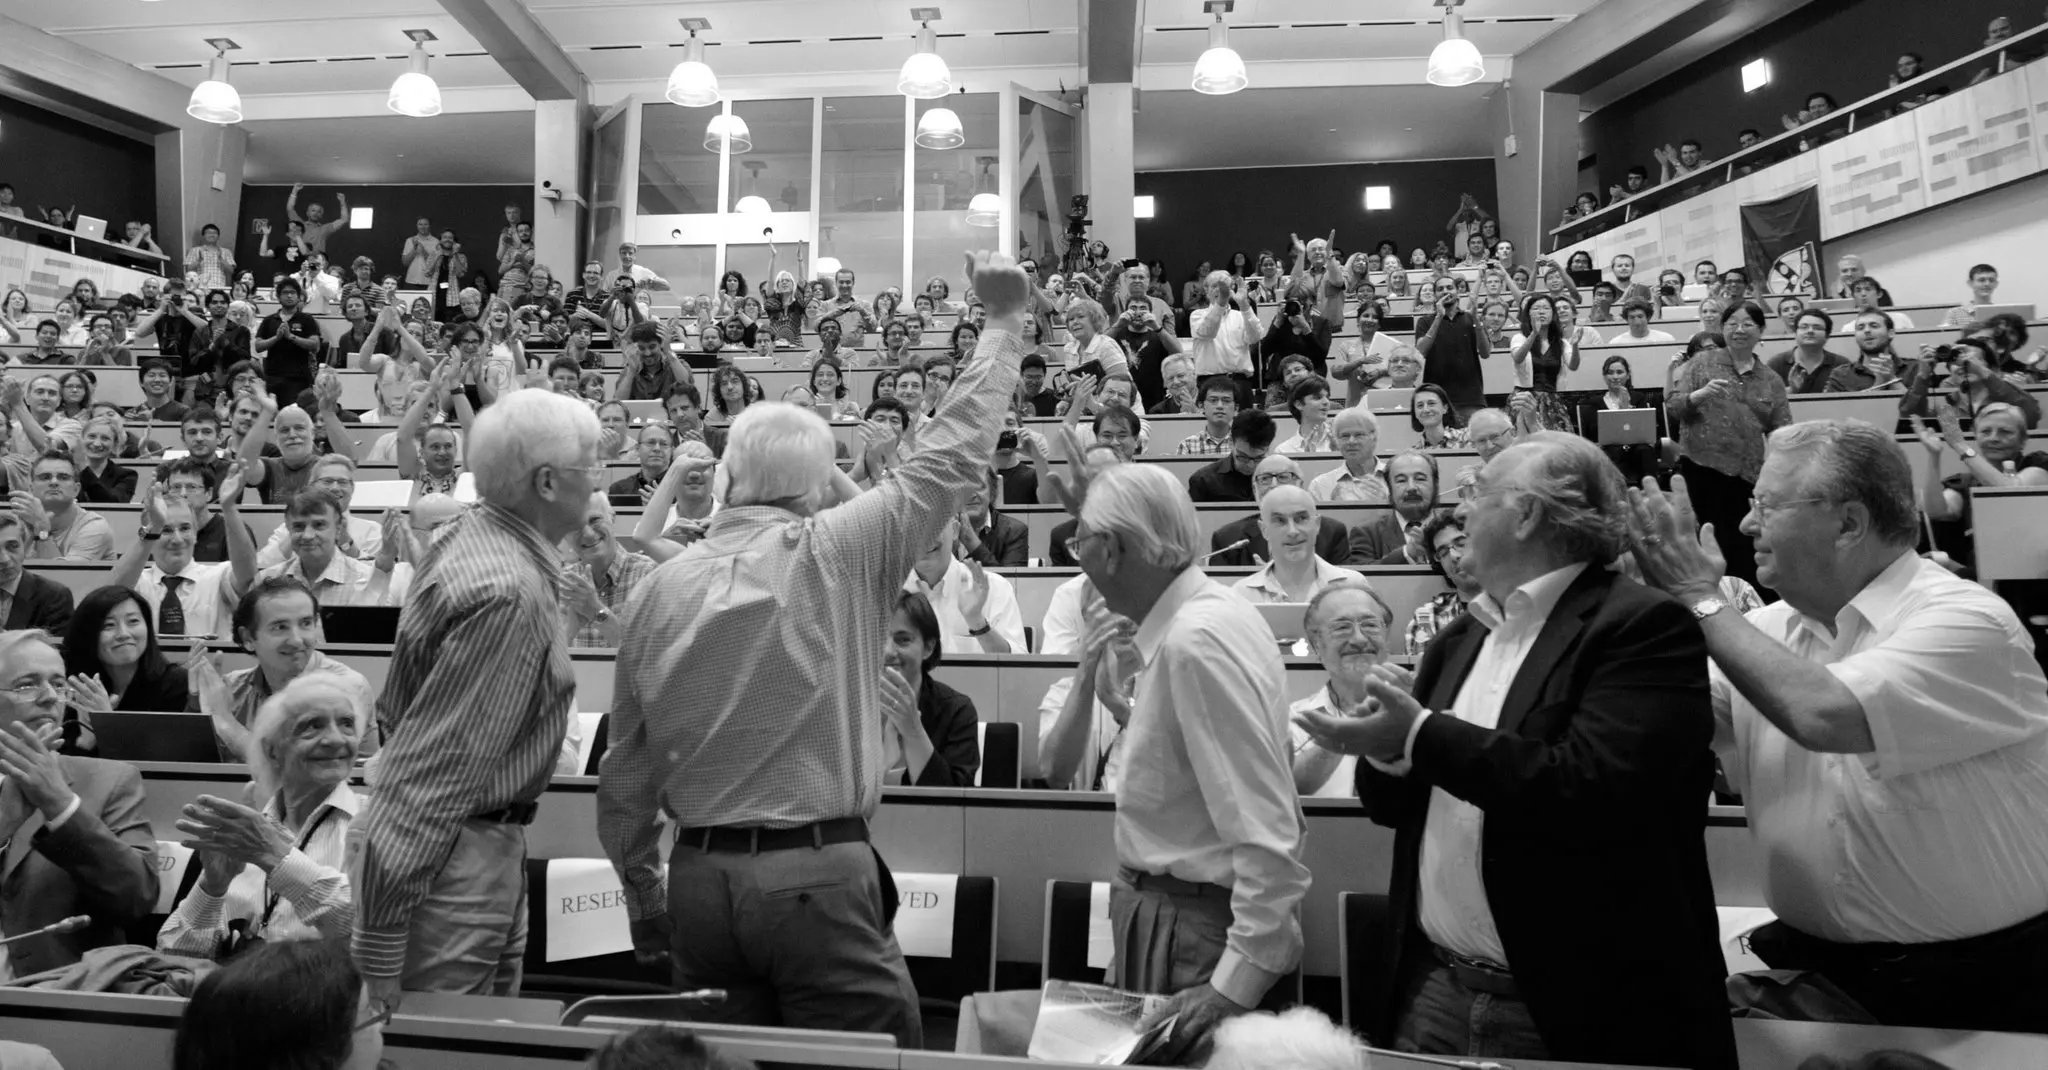
\includegraphics[width=0.5\textwidth]{./figures/HiggsBosonDiscoveryBW.png}
      \end{center}
    \end{figure}
    % ========================
  \end{multicols}
\end{MyArticle}

        \begin{MyArticle}[enhanced, tikz={rotate=0}]{Top Quark, Last Piece of Matter, Appears to Be in Place}
  \begin{multicols}{2}
    We establish the existence of the top quark using a 67 pb$^{-1}$ data
    sample of pp collisions at $\sqrt{s} = 1.8$ TeV collected with the Collider
    Detector at Fermilab (CDF). Employing techniques similar to those we
    previously published, we observe a signal consistent with $t\bar{t}$ decay to
    $WWbb$, but inconsistent with the background prediction by
    4.8$\sigma$. Additional evidence for the top quark is provided by a peak in
    the reconstructed mass distribution. We measure the top quark mass
    to be $176 \pm 8 (\text{stat.}) \pm 10 (\text{sys.})$ GeV/c$^{2}$,
    and the $t\bar{t}$ production cross section to be
    $6.8^{+3.6}_{-2.4}$ pb.
    % ========================
    \begin{figure}
      \begin{center}
        \vspace{-0.2in}
        \leavevmode
        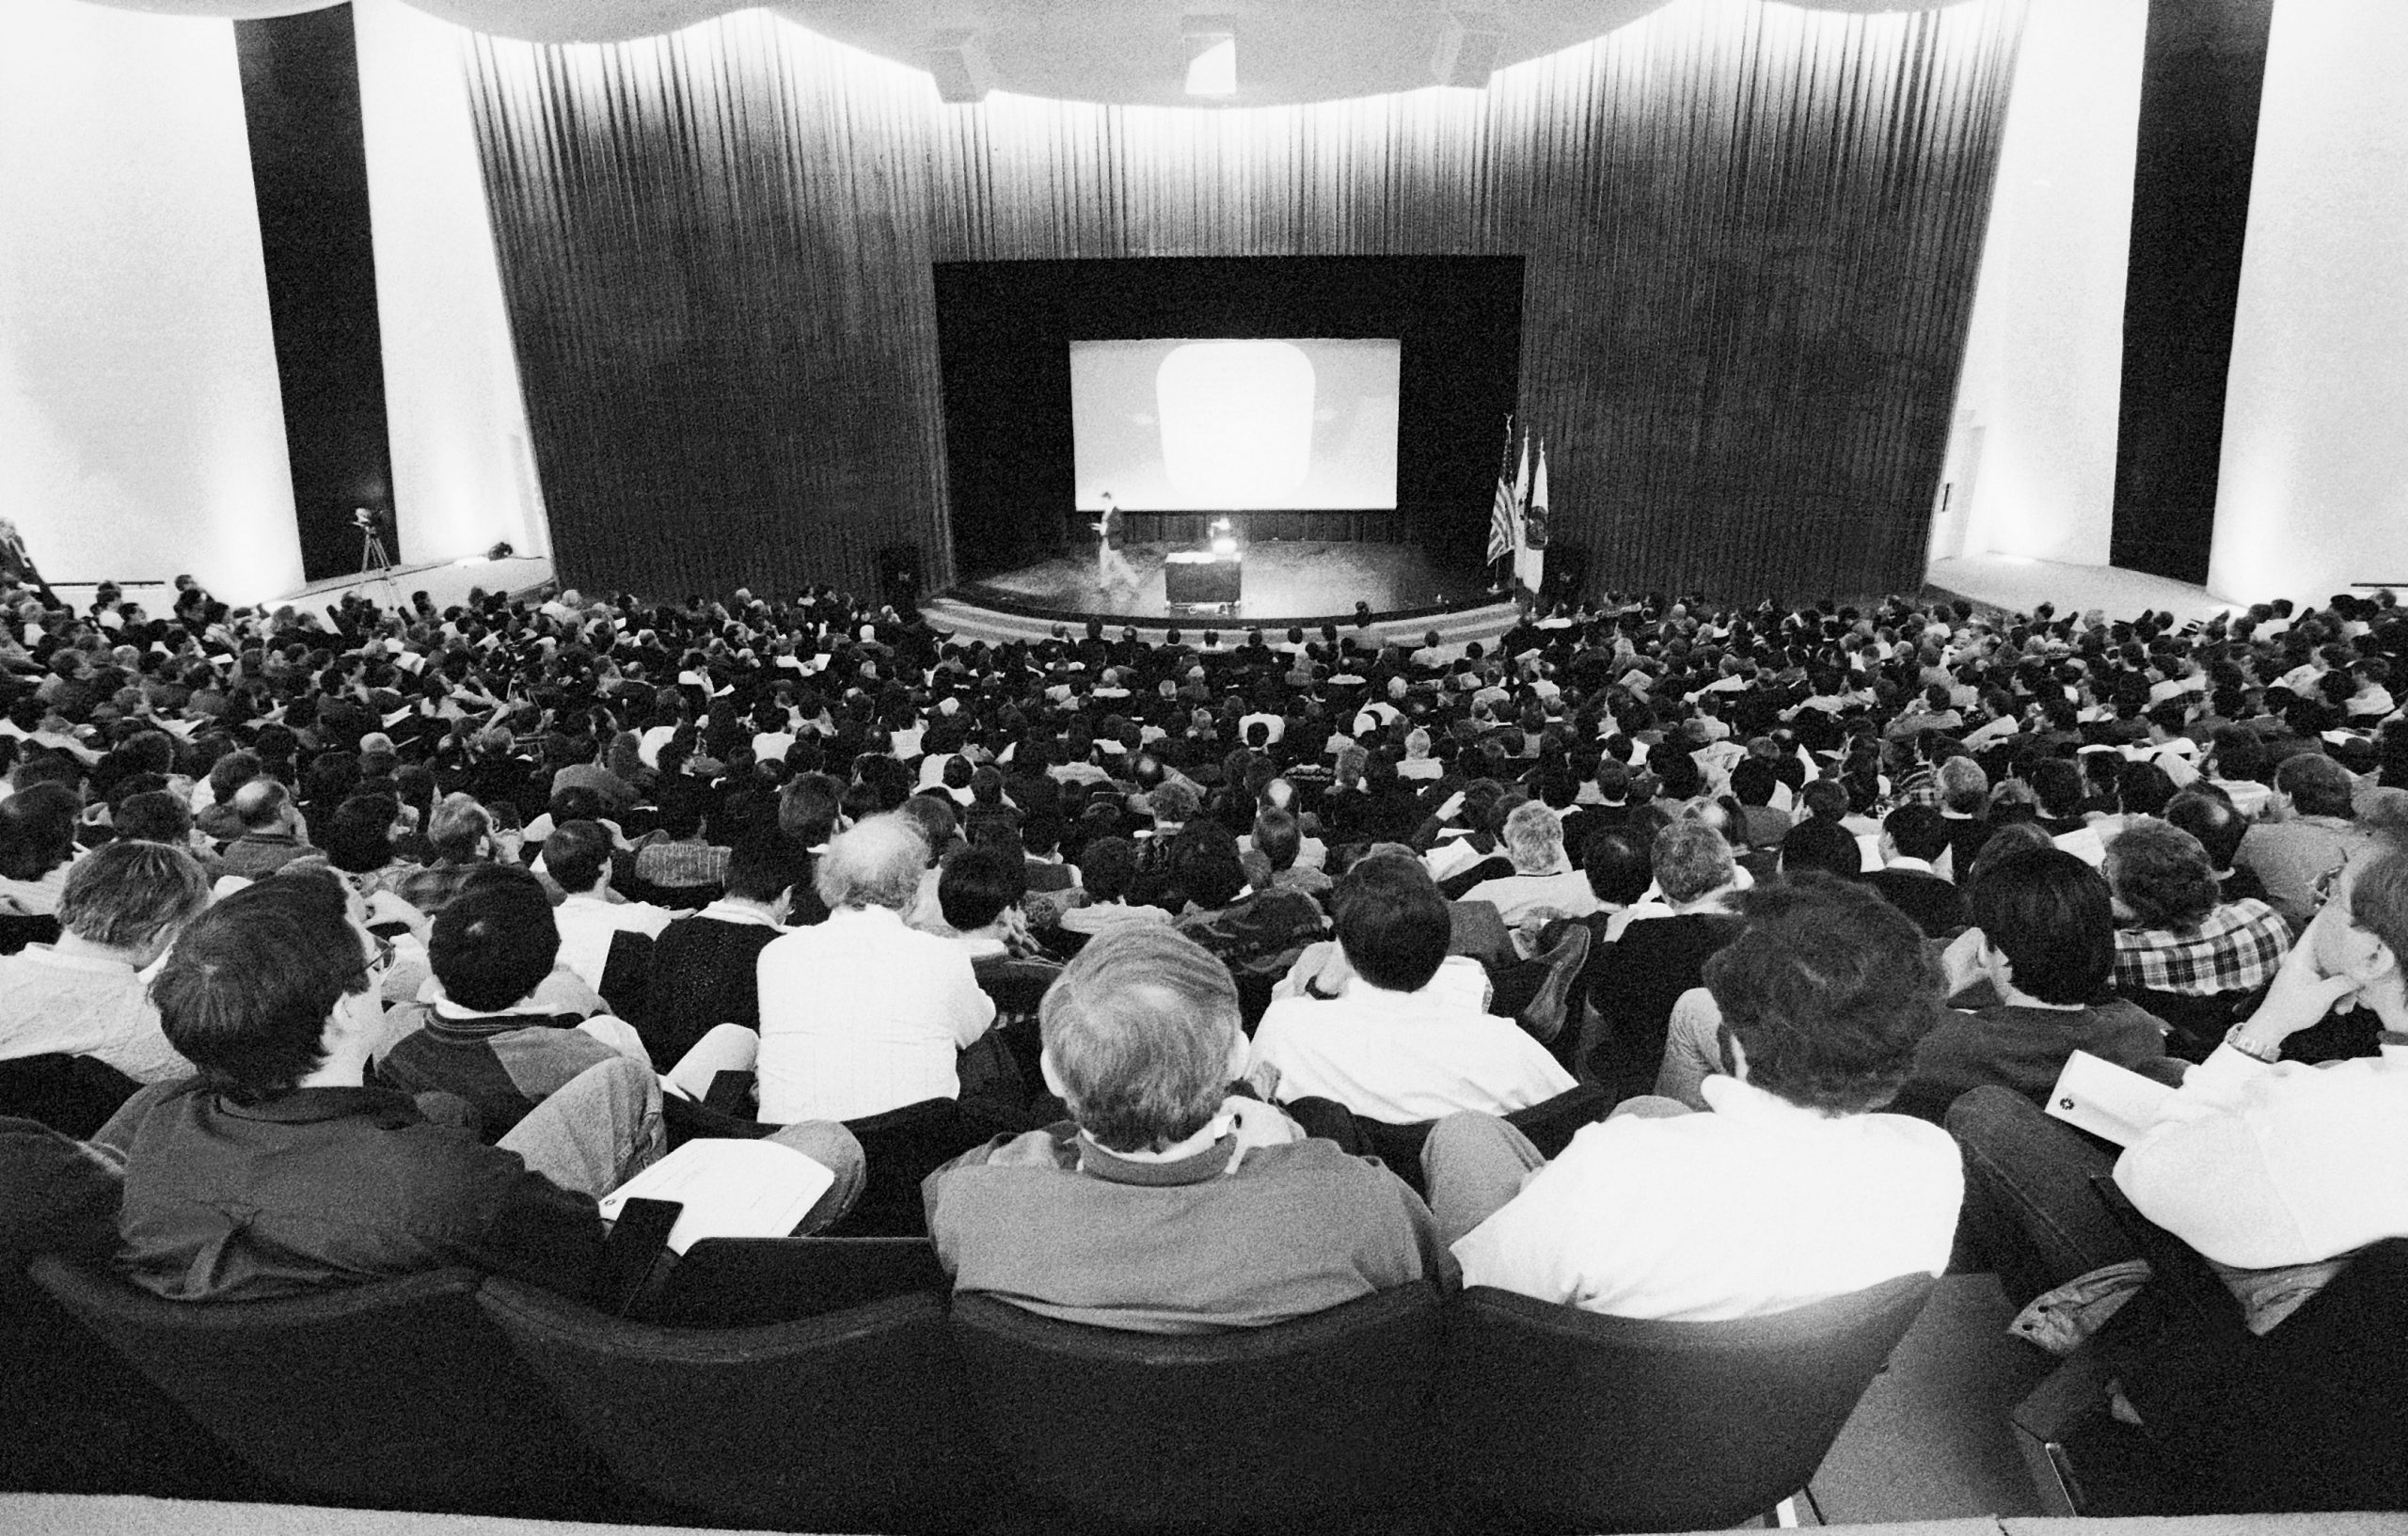
\includegraphics[width=0.5\textwidth]{./figures/TopQuarkAnnouncement.jpg}
      \end{center}
    \end{figure}
    % ========================
  \end{multicols}
\end{MyArticle}

      \end{column}
      \begin{column}{0.5\paperwidth} \begin{headline}[enhanced, tikz={rotate=0}]{Fotios Ptochos Promoted to Professor!}
  % https://www.overleaf.com/learn/latex/Multiple_columns
  \begin{multicols}{2}
    Congratulations to Fotios Ptochos for his promotion to the rank of
    Full Professor, effective November 2022. This promotion recognizes
    Prof. Ptochos' achievements in scholarship, teaching in physics and research in
    high-energy physics (HEP), and his overall service to the CDF and CMS
    Collaborations. He is a Harvard University PhD in physics
    graduate (1998) and has been active in HEP-research, both in detector
    development and physics analyses since 1987. In particular, from 1987
    to 1988 he worked in the development of a technique to monitor the
    purity of Liquid Argon (LAr) for the first ever prototype of the
    ICARUS detector, a technique that was subsequently used in the
    experiment. From 1989 to 1994 he worked in the characterization of
    various Tetramethyl liquids as part of a research project to find
    appropriate warm liquids media for the envisioned calorimeter
    detectors at SSC. He also worked in the construction, installation and
    calibration of the Central Muon Extension (CMX) system for the CDF
    detector. From 1994 to 1996 he developed an algorithm to improve
    electron identification for the CDF end-plug ECAL based on the
    information from the calorimeter and hits on the silicon tracker
    detector. The algorithm led to the development and implementation of
    the PHOENIX tracker system in the CDF-II detector. 
    In the period of 2000–2003, he was the coordinator of the group
    responsible for the development, installation, maintenance and
    performance monitoring of the CDF-II Hadronic Calorimeter (HCAL)
    timing system. For the entire period of the Tevatron Run-II
    (2001-2011) he served as the coordinator of the CDF central HCAL
    calibration (CHA and WHA), maintenance and performance group. Since
    2004, when he joined the faculty of the UCY Physics Department, he has
    been involved in the UCY HEP group activities related to the
    construction and running of the CMS ECAL at CERN. In 2009, he
    initiated the involvement of the group in the activities related to
    the CMS tracking detector. He was also involved in the development of
    the dual-readout calorimetry concept in a total absorption HCAL for
    future linear-collider experiments. 
    Professor Ptochos has led numerous physics analyses, spanning
    from precision measurements on properties of heavy flavour quark
    production and their use as probes for searching for the SM and SUSY
    Higgs bosons, to searches for BSM physics including SUSY, extra
    dimensions and other exotic processes. He has tremendous experience in
    heavy flavour tagging techniques and algorithms, tau-lepton
    identification techniques and new physics model building. 
    He was the first ever recipient of the \say{Fermi National
      Accelerator Laboratory Fellowship} and has co-coordinated multiple research program
    funded primarily by the European Commission (EC) via \textsc{Marie
    Skłodowska-Curie Actions},  the Cyprus Research Promotion
    Foundation (RPF) through \textsc{Didaktor} or \textsc{Excellence
      Hubs} programs, the European Regional Development Fund, and
    UCY. Professor Ptochos is the author and co-author of more than 
    1700 publications in refereed scientific journals and a member of the
    editorial group in charge for producing the education material
    for the entire Cyprus Secondary Education. In addition, he has
    been the supervisor of the research activities of six postdoctoral
    fellows, five PhD and eleven MSc students, as well as the theses
    projects of more than 20 undergraduate students. 

    % ========================
    \begin{figure}
      \begin{center}
        \vspace{-0.2in}
        \leavevmode
        \includegraphics[width=0.5\textwidth]{./figures/Fotis6.png}
      \end{center}
    \end{figure}
    % ========================
  \end{multicols}
\end{headline}
 \end{column}
      \begin{column}{0.25\paperwidth} %\begin{MyArticle}[enhanced, height=0.2\textheight,
%tikz={rotate=0}]{Physicists Find Elusive Particle Seen as Key to
%Universe}
\begin{MyArticle}[enhanced, tikz={rotate=0}, width=0.35\textwidth]{Physicists Find Elusive Particle Seen as Key to Universe}
  \begin{multicols}{2}
    Results are presented from searches for the standard model Higgs
    boson in proton–proton collisions at and 8 TeV in the Compact Muon
    Solenoid experiment at the LHC, using data samples corresponding
    to integrated luminosities of up to 5.1 fb$^{−1}$ at 7 TeV and 5.3 fb$^{−1}$
    at 8 TeV. The search is performed in five decay modes:
    $\gamma\gamma$, $ZZ$,  $\tau^{+}\tau^{-}$, and $b\bar{b}$.
    An excess of events is observed above the expected background,
    with a local significance of 5.0 standard deviations, at a mass
    near 125 GeV, signalling the production of a new particle. The
    expected significance for a standard model Higgs boson of that
    mass is 5.8 standard deviations. The excess is most significant in
    the two decay modes with the best mass resolution, $\gamma\gamma$ and $ZZ$; a
    fit to these signals gives a mass of 
    $125.3\pm0.4(\text{stat.})\pm0.5(\text{syst.}$ GeV. The decay to
    two photons indicates that the new particle is a boson with spin 
    different from one. 
    % ========================
    \begin{figure}
      \begin{center}
        \vspace{-0.2in}
        \leavevmode
        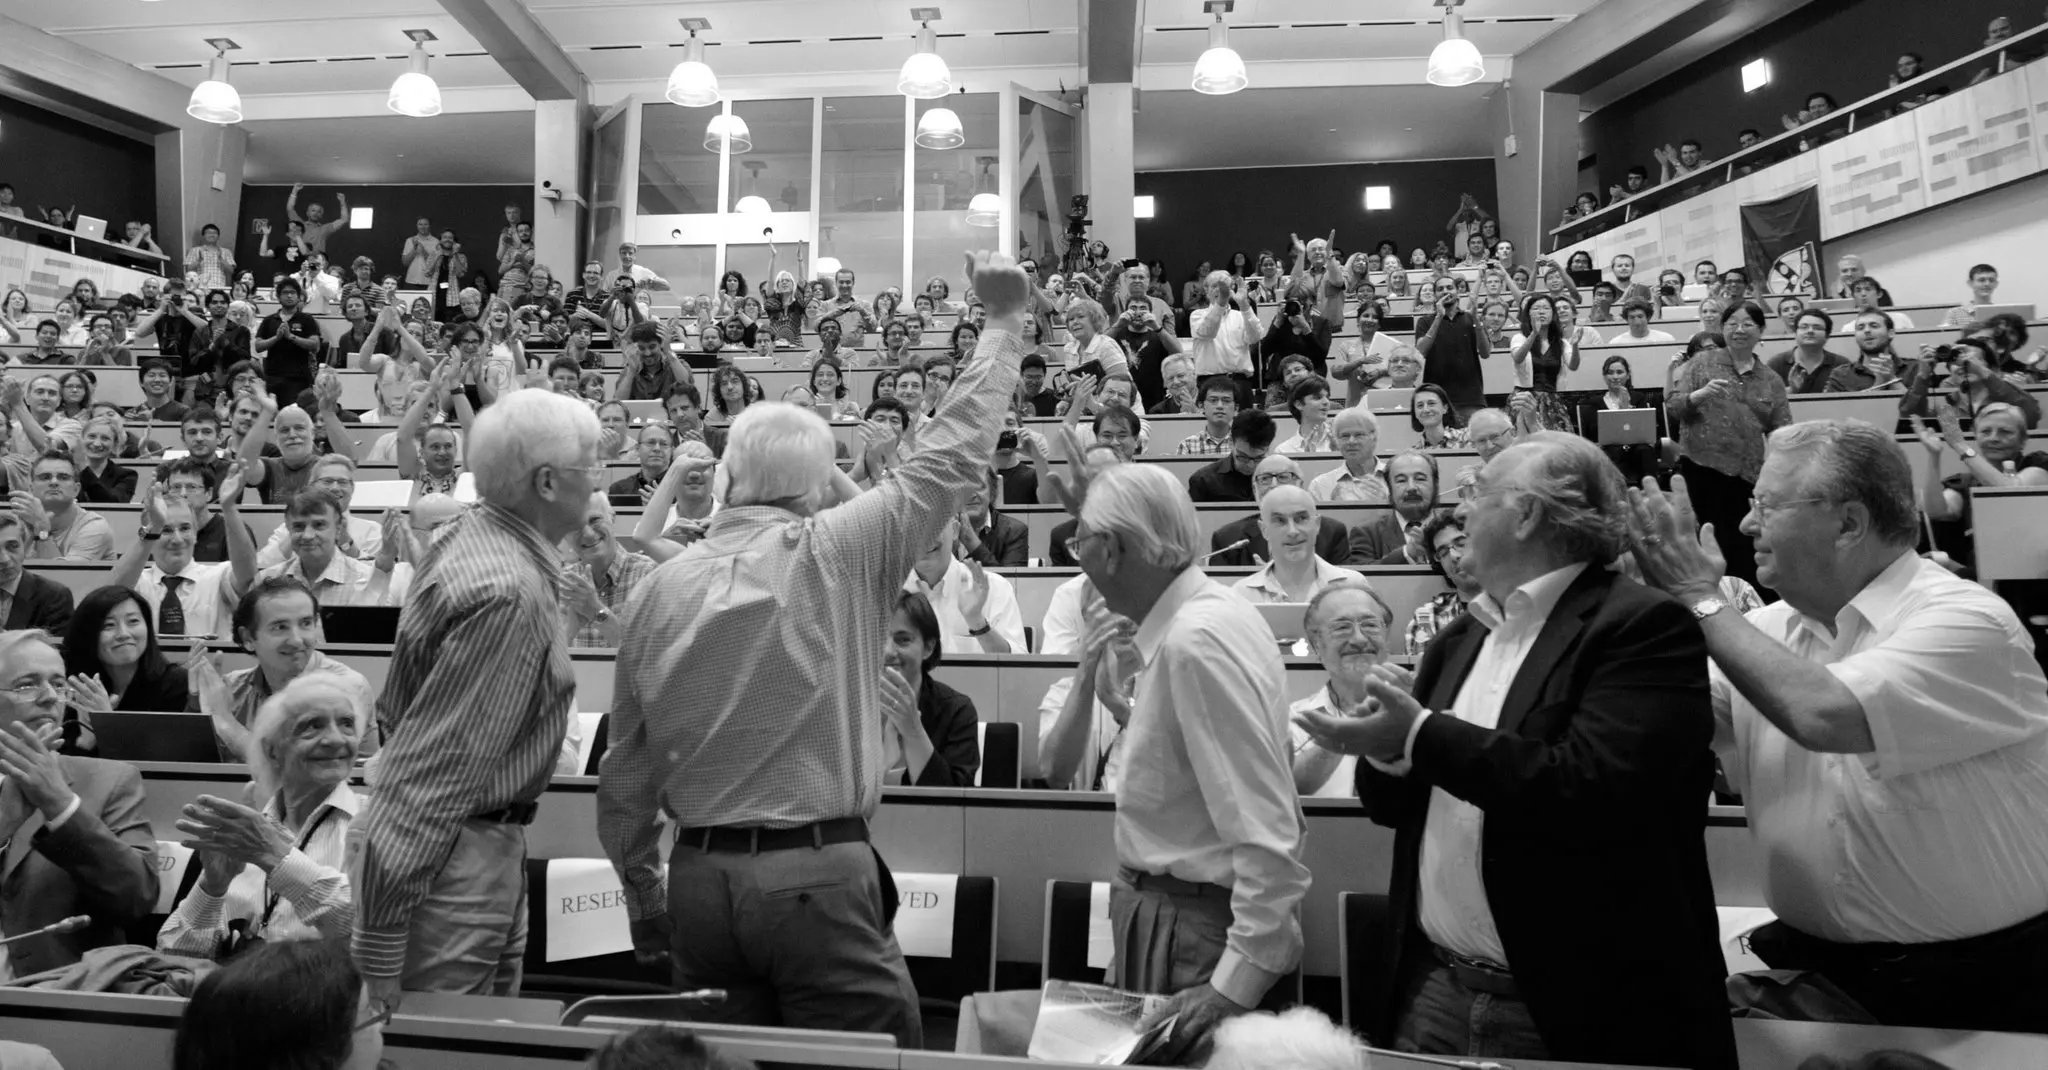
\includegraphics[width=0.5\textwidth]{./figures/HiggsBosonDiscoveryBW.png}
      \end{center}
    \end{figure}
    % ========================
  \end{multicols}
\end{MyArticle}
 \end{column}
    \end{columns}
  \end{columns}


\begin{columns}[t]
    \begin{columns}[t,totalwidth=1.0\paperwidth] % split up that three-column-wide column
      \begin{column}{0.2\paperwidth} \begin{MyArticle}[enhanced, tikz={rotate=0}, boxrule=1pt,
  titlerule=0pt, width=0.33\textwidth]{CDF publishes multi-muons!}
  \begin{multicols}{2}
    We report a study of multi-muon events produced at the
    Fermilab Tevatron collider and recorded by the CDF~II detector. In a data 
    set acquired with a dedicated dimuon trigger and corresponding to an 
    integrated luminosity of 2100 pb$^{-1}$, we isolate a significant sample of 
    events in which at least one of the muon candidates is produced 
    outside of the beam pipe of radius 1.5 cm. The production cross section
    and kinematics of events in which both muon candidates are produced inside
    the beam pipe are successfully modeled by known QCD processes which
    include heavy flavor production. In contrast, we are presently unable to 
    fully account for the number and properties of the remaining events, in which
    at least one muon candidate is produced outside of the beam pipe, in terms
    of the same understanding of the CDF~II detector, trigger, and event 
    reconstruction. Several topological and kinematic properties of these 
    events are presented in this paper. These events offer a plausible 
    resolution to long-standing inconsistencies related to $b\bar{b}$
    production and decay.
    \begin{comment}
    % ========================
    \begin{figure}
      \begin{center}
        \vspace{-0.2in}
        \leavevmode
        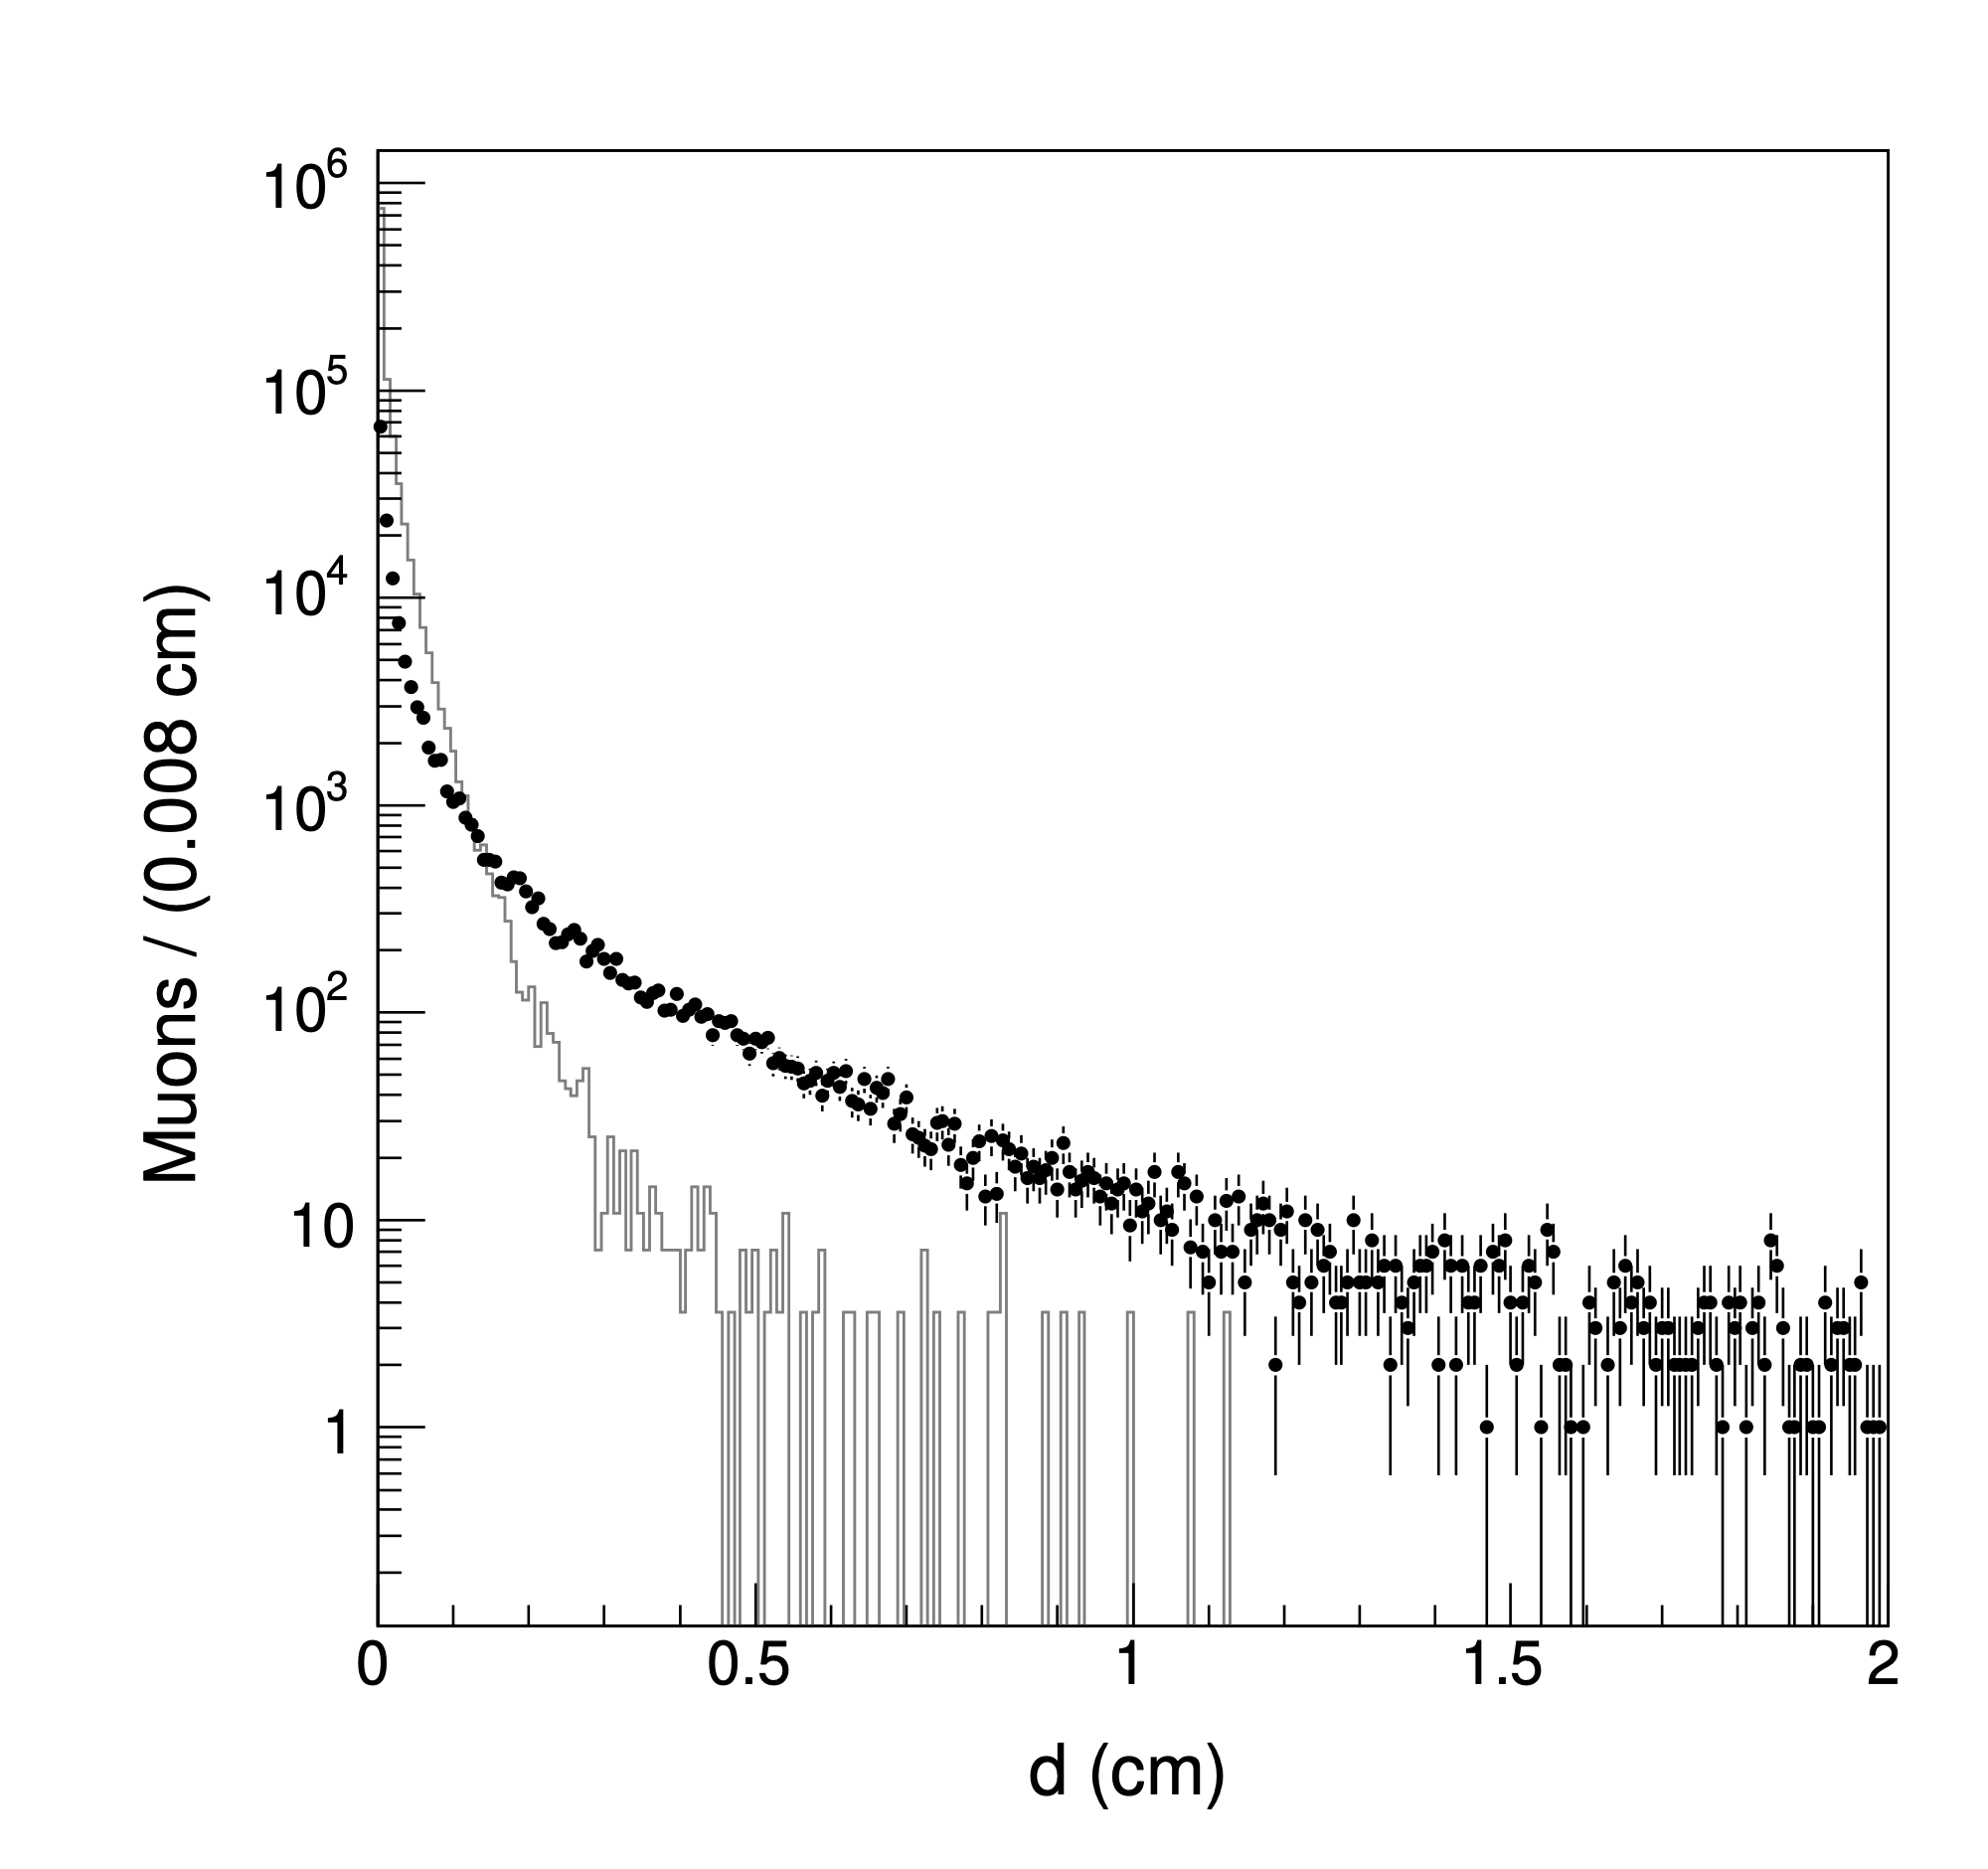
\includegraphics[width=\textwidth]{./figures/MultiMuons1BW_CDF.png}
        %\caption[] {Impact parameter distribution of muons contributed by ghost
        %  ($\bullet$) and QCD (histogram) events. Muon tracks are
        %  selected with loose SVX requirements. The detector resolution
        %  is $\simeq 30 \; \mu$m, whereas bins are 80 $\mu$m wide.} 
      \end{center}
    \end{figure}
    % ========================
    \end{comment}
  \end{multicols}
\end{MyArticle}
 \end{column}
      \begin{column}{0.2\paperwidth} \begin{multimuons-2}[enhanced, tikz={rotate=0}]{Multi-Muons In CDF: The Mystery Continues}
  %\begin{multicols}{2}
    We present a phenomenological conjecture of new physics that is suggested
    by the topology and kinematic properties of the multi-muon events recently
    reported by the CDF collaboration. We show that the salient features of 
    the data can be accounted for by postulating the pair production of
    three new states $h_1$, $h_2$, and $h_3$ with masses in the range
    of 15, 7.3, and 3.6 GeV/c$^{2}$, respectively. The heavier states 
    cascade-decay into the lighter ones, whereas the lightest state 
    decays into a $\tau$ pair with a lifetime of the order of 20 ps.
    \begin{comment}
    % ========================
    \begin{figure}
      \begin{center}
        \vspace{-0.2in}
        \leavevmode
        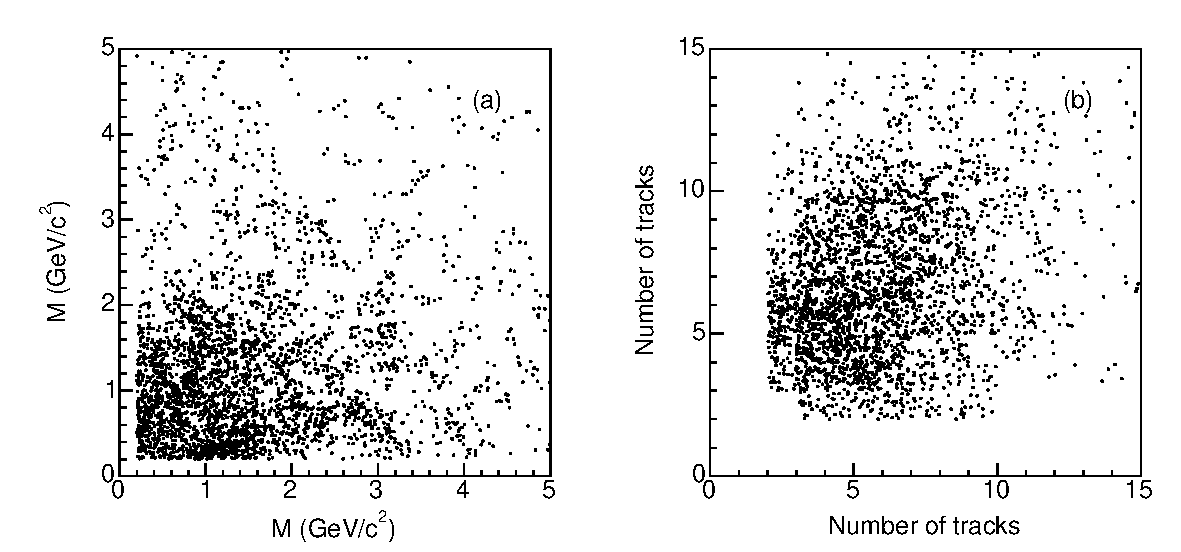
\includegraphics[width=\textwidth]{./figures/MultiMuons2_CDF.pdf}
        %\caption[]{Two-dimensional distributions, reproduced from Ref.~\cite{a0disc},
        %  of (a) the invariant mass, $M$, of all muons and (b) the total
        %  number of tracks contained in a $36.8^{\deg}$ cone when both
        %  cones contain at least two muons.}
      \end{center}
    \end{figure}
    % ========================
    \end{comment}
%  \end{multicols}
\end{multimuons-2}
 \end{column}
      \begin{column}{0.2\paperwidth} \begin{MyArticle}[enhanced, tikz={rotate=0}, width=0.25\textwidth]{Charged Higgs boson
    Hunting}
  $t\rightarrow bH^{\pm}\rightarrow \tau^{\pm} \nu_{\tau}$............................\it{25 May 2012}\newline
  $H^{\pm}\rightarrow tb$ and $H^{\pm}\rightarrow \tau\nu$..............\it{31 August 2015}\newline
  $H^{\pm} \rightarrow \tau^{\pm} \nu_{\tau}$ ................................\it{11 March 2019}\newline
  $pp\rightarrow t(b)H^{\pm} \rightarrow tb$, all-jet.......\it{21 January 2020}\newline
  $pp\rightarrow t(b)H^{\pm} \rightarrow W^{\pm}H^{0}(\tau\tau)$...............\it{4 July 2022}
  %\begin{tabular}{l l}
%  \hline
%  \bf $H^{\pm} \rightarrow \tau^{\pm} \nu_{\tau}$  & \it{11 March 2019}\\
%  \bf $H^{\pm} \rightarrow tb$, all-jet            & \it{21 January 2020}\\
%  \bf $H^{\pm} \rightarrow W^{\pm}H^{0}(\tau\tau)$ & \it{4 July 2022}\\
%  \hline
%\end{tabular}
\end{MyArticle}
% https://cms-results.web.cern.ch/cms-results/public-results/publications/HIG-11-019/index.html
% https://cms-results.web.cern.ch/cms-results/public-results/publications/HIG-14-023/index.html
% https://cms-results.web.cern.ch/cms-results/public-results/publications/HIG-18-014/index.html
% https://cms-results.web.cern.ch/cms-results/public-results/publications/HIG-18-015/index.html
% https://cms-results.web.cern.ch/cms-results/public-results/publications/HIG-21-010/index.html


\begin{comment}
\begin{multimuons-1}[enhanced, tikz={rotate=0}, width=1.0\textwidth]{\huge Charged Higgs boson Hunting}

  \Large{$t\rightarrow bH^{\pm}\rightarrow \tau^{\pm} \nu_{\tau}$}............................\it{\Large 25 May 2012}\newline
  \Large{$H^{\pm}\rightarrow tb$ and $H^{\pm}\rightarrow \tau\nu$}..............\it{\Large 31 August 2015}\newline
  \Large{$H^{\pm} \rightarrow \tau^{\pm} \nu_{\tau}$}................................\it{\Large 11 March 2019}\newline
  \Large{$pp\rightarrow t(b)H^{\pm} \rightarrow tb$, all-jet}.......\it{\Large 21 January 2020}\newline
  \Large{$pp\rightarrow t(b)H^{\pm} \rightarrow W^{\pm}H^{0}(\tau\tau)$}...............\it{\Large 4 July 2022}
\end{multimuons-1}
\end{comment}
 \end{column}
      \begin{column}{0.2\paperwidth} % https://gitlab.cern.ch/tdr/papers/HIG-21-010/-/tree/master/
% new tcolorbox environment
\newtcolorbox{topQuark}[2][]{
  coltext      = black,
  colframe     = \MyBlockFrameColorLeft,
  colback      = \MyBlockFillColorLeft,
  colbacktitle = \MyBlockTitleBoxColor,
  coltitle     = black,
  title        = {\Large{\textbf{#2}}},
  fonttitle    = \bfseries,
  boxrule      = 0.2cm, %frame line width
  top=+0.0cm, bottom=+0.0cm, left=+0.05cm, right=+0.05cm,
  opacityback=1.0, % 1.0 means totally transparent, 0.0 means totally opaque
  arc=0.0cm,        % 0.0cm for non-rounded corners!
  #1,
}

% CMS
\begin{topQuark}[enhanced, tikz={rotate=0}]{Search for charged Higgs bosons decaying into a top and a bottom quark in the all-jet final state}
    A search for charged Higgs bosons ($H^{\pm}$) decaying into a top
    and a bottom quark in the all-jet final state is presented. The
    analysis uses LHC proton-proton collision data recorded with the
    CMS detector in 2016 at $\sqrt{s} = 13$ TeV, corresponding to an
    integrated luminosity of 35.9~$fb^{-1}$. No significant excess is
    observed above the expected background. Model-independent upper
    limits at 95$\%$ confidence level are set on the product of the
    $H^{\pm}$ production cross section and branching fraction in two
    scenarios.  For production in association with a top quark,
    limits of 21.3 to 0.007$pb$ are obtained for $H^{\pm}$ masses in the
    range of 0.2 to 3 TeV. Combining this with a search in leptonic
    final states results in improved limits of 9.25 to 0.005 $pb$. The
    complementary $s$-channel production of an $H^{\pm}$ is
    investigated in the mass range of 0.8 to 3 TeV and the
    corresponding upper limits are 4.5 to 0.023 $pb$. These results are
    interpreted using different minimal supersymmetric extensions of
    the standard model.
\end{topQuark}
\end{column} 
      \begin{column}{0.2\paperwidth} % https://gitlab.cern.ch/tdr/papers/HIG-21-010/-/tree/master/
% new tcolorbox environment
\newtcolorbox{topQuark}[2][]{
  coltext      = black,
  colframe     = \MyBlockFrameColorLeft,
  colback      = \MyBlockFillColorLeft,
  colbacktitle = \MyBlockTitleBoxColor,
  coltitle     = black,
  title        = {\Large{\textbf{#2}}},
  fonttitle    = \bfseries,
  boxrule      = 0.2cm, %frame line width
  %tikz={rotate=#3}, % manipulate the tcolorbox as a whole (in degrees)
  top=+0.0cm, bottom=+0.0cm, left=+0.05cm, right=+0.05cm,
  %enlarge top by   = +1.0cm,  %  equivalent to mdframed 'skipabove'
  %enlarge bottom by= +0.0cm,  %  equivalent to mdframed 'skipbelow'
  %enlarge left by  = +1.5cm,  
  %enlarge right by = +0.0cm, 
  opacityback=1.0, % 1.0 means totally transparent, 0.0 means totally opaque
  arc=0.0cm,        % 0.0cm for non-rounded corners!
  #1,
}

% CMS
\begin{topQuark}[enhanced, tikz={rotate=0}]{Higgs boson: a tool to
    discover new physics: $H^{\pm}$}
  \begin{multicols}{2}
  A search for a charged Higgs boson $H^{\pm}$ decaying
  into a heavy neutral Higgs boson $H$ and a $W$ boson
  is presented. The analysis targets the $W$ decay into a pair
  of tau leptons with at least one of them decaying hadronically and
  with an additional electron or muon present in the event.
  The search is based on proton-proton collision data
  recorded by the CMS experiment during 2016--2018 at
  $\sqrt{s} = 13~TeV$, corresponding to an integrated
  luminosity of 138~$fb^{-1}$. The data are consistent with
  standard model background expectations. Upper limits at 95$\%$ confidence
  level are set on the product of the cross section and branching fraction
  for an $H^{\pm}$ in the mass range of 300--700 GeV, assuming an $H$ 
  with a mass of 200 GeV. The observed limits range from
  0.085 $pb$ for an $H^{\pm}$ mass of
  300 $GeV$ to 0.019~$pb$ for a mass of
  700 $GeV$. These are the first limits on $H^{\pm}$
  production in the $H^{\pm} \to H W^{\pm}$ decay channel at the LHC.
  \end{multicols}
\end{topQuark}
 \end{column}
    \end{columns}
\end{columns}

%\begin{columns}[t]
%  \begin{columns}[t,totalwidth=1.0\paperwidth] % split up that three-column-wide column
%  \end{columns}
%\end{columns}



\begin{comment}
\begin{columns}[t]
    \begin{columns}[t,totalwidth=1.0\paperwidth] % split up that three-column-wide column
      \begin{column}{0.25\paperwidth} \begin{MyArticle}[enhanced, tikz={rotate=0}, width=0.25\textwidth]{Charged Higgs boson
    Hunting}
  $t\rightarrow bH^{\pm}\rightarrow \tau^{\pm} \nu_{\tau}$............................\it{25 May 2012}\newline
  $H^{\pm}\rightarrow tb$ and $H^{\pm}\rightarrow \tau\nu$..............\it{31 August 2015}\newline
  $H^{\pm} \rightarrow \tau^{\pm} \nu_{\tau}$ ................................\it{11 March 2019}\newline
  $pp\rightarrow t(b)H^{\pm} \rightarrow tb$, all-jet.......\it{21 January 2020}\newline
  $pp\rightarrow t(b)H^{\pm} \rightarrow W^{\pm}H^{0}(\tau\tau)$...............\it{4 July 2022}
  %\begin{tabular}{l l}
%  \hline
%  \bf $H^{\pm} \rightarrow \tau^{\pm} \nu_{\tau}$  & \it{11 March 2019}\\
%  \bf $H^{\pm} \rightarrow tb$, all-jet            & \it{21 January 2020}\\
%  \bf $H^{\pm} \rightarrow W^{\pm}H^{0}(\tau\tau)$ & \it{4 July 2022}\\
%  \hline
%\end{tabular}
\end{MyArticle}
% https://cms-results.web.cern.ch/cms-results/public-results/publications/HIG-11-019/index.html
% https://cms-results.web.cern.ch/cms-results/public-results/publications/HIG-14-023/index.html
% https://cms-results.web.cern.ch/cms-results/public-results/publications/HIG-18-014/index.html
% https://cms-results.web.cern.ch/cms-results/public-results/publications/HIG-18-015/index.html
% https://cms-results.web.cern.ch/cms-results/public-results/publications/HIG-21-010/index.html


\begin{comment}
\begin{multimuons-1}[enhanced, tikz={rotate=0}, width=1.0\textwidth]{\huge Charged Higgs boson Hunting}

  \Large{$t\rightarrow bH^{\pm}\rightarrow \tau^{\pm} \nu_{\tau}$}............................\it{\Large 25 May 2012}\newline
  \Large{$H^{\pm}\rightarrow tb$ and $H^{\pm}\rightarrow \tau\nu$}..............\it{\Large 31 August 2015}\newline
  \Large{$H^{\pm} \rightarrow \tau^{\pm} \nu_{\tau}$}................................\it{\Large 11 March 2019}\newline
  \Large{$pp\rightarrow t(b)H^{\pm} \rightarrow tb$, all-jet}.......\it{\Large 21 January 2020}\newline
  \Large{$pp\rightarrow t(b)H^{\pm} \rightarrow W^{\pm}H^{0}(\tau\tau)$}...............\it{\Large 4 July 2022}
\end{multimuons-1}
\end{comment}
 \end{column}
      \begin{column}{0.75\paperwidth} % new tcolorbox environment
\newtcolorbox{headline}[2][]{
  coltext      = black,
  colframe     = \MyBlockFrameColorLeft,
  colback      = \MyBlockFillColorLeft,
  colbacktitle = \MyBlockTitleBoxColor,
  coltitle     = black,
  title        = {\Huge{\textbf{#2}}},
  fonttitle    = \bfseries,
  boxrule      = 0.2cm, %frame line width
  %tikz={rotate=#3}, % manipulate the tcolorbox as a whole (in degrees)
  top=+0.0cm, bottom=+0.0cm, left=+0.05cm, right=+0.05cm,
  %enlarge top by   = +1.0cm,  %  equivalent to mdframed 'skipabove'
  %enlarge bottom by= +0.0cm,  %  equivalent to mdframed 'skipbelow'
  %enlarge left by  = +1.5cm,  
  %enlarge right by = +0.0cm, 
  opacityback=1.0, % 1.0 means totally transparent, 0.0 means totally opaque
  arc=0.0cm,        % 0.0cm for non-rounded corners!
  #1,
}

% CMS
\begin{headline}[enhanced, tikz={rotate=0}]{Fotios Ptochos Promoted to Professor!}
  \begin{multicols}{2}
    \lipsum[1]\\ 
    \lipsum[2]\\ 
    %\lipsum[3]\\ 
    % ========================
    \begin{figure}
      \begin{center}
        \vspace{-0.2in}
        \leavevmode
        \includegraphics[width=0.5\textwidth]{./figures/Fotis6.png}
      \end{center}
    \end{figure}
    % ========================
  \end{multicols}
\end{headline}
 \end{column}
    \end{columns}
  \end{columns}

\begin{columns}[t]
    \begin{columns}[t,totalwidth=1.0\paperwidth] % split up that three-column-wide column
      \begin{column}{0.35\paperwidth} % https://gitlab.cern.ch/tdr/papers/HIG-21-010/-/tree/master/
% new tcolorbox environment
\newtcolorbox{topQuark}[2][]{
  coltext      = black,
  colframe     = \MyBlockFrameColorLeft,
  colback      = \MyBlockFillColorLeft,
  colbacktitle = \MyBlockTitleBoxColor,
  coltitle     = black,
  title        = {\Large{\textbf{#2}}},
  fonttitle    = \bfseries,
  boxrule      = 0.2cm, %frame line width
  top=+0.0cm, bottom=+0.0cm, left=+0.05cm, right=+0.05cm,
  opacityback=1.0, % 1.0 means totally transparent, 0.0 means totally opaque
  arc=0.0cm,        % 0.0cm for non-rounded corners!
  #1,
}

% CMS
\begin{topQuark}[enhanced, tikz={rotate=0}]{Search for charged Higgs bosons decaying into a top and a bottom quark in the all-jet final state}
    A search for charged Higgs bosons ($H^{\pm}$) decaying into a top
    and a bottom quark in the all-jet final state is presented. The
    analysis uses LHC proton-proton collision data recorded with the
    CMS detector in 2016 at $\sqrt{s} = 13$ TeV, corresponding to an
    integrated luminosity of 35.9~$fb^{-1}$. No significant excess is
    observed above the expected background. Model-independent upper
    limits at 95$\%$ confidence level are set on the product of the
    $H^{\pm}$ production cross section and branching fraction in two
    scenarios.  For production in association with a top quark,
    limits of 21.3 to 0.007$pb$ are obtained for $H^{\pm}$ masses in the
    range of 0.2 to 3 TeV. Combining this with a search in leptonic
    final states results in improved limits of 9.25 to 0.005 $pb$. The
    complementary $s$-channel production of an $H^{\pm}$ is
    investigated in the mass range of 0.8 to 3 TeV and the
    corresponding upper limits are 4.5 to 0.023 $pb$. These results are
    interpreted using different minimal supersymmetric extensions of
    the standard model.
\end{topQuark}
\end{column} 
      \begin{column}{0.35\paperwidth}  %\begin{MyArticle}[enhanced, height=0.2\textheight,
%tikz={rotate=0}]{Physicists Find Elusive Particle Seen as Key to
%Universe}
\begin{MyArticle}[enhanced, tikz={rotate=0}, width=0.35\textwidth]{Physicists Find Elusive Particle Seen as Key to Universe}
  \begin{multicols}{2}
    Results are presented from searches for the standard model Higgs
    boson in proton–proton collisions at and 8 TeV in the Compact Muon
    Solenoid experiment at the LHC, using data samples corresponding
    to integrated luminosities of up to 5.1 fb$^{−1}$ at 7 TeV and 5.3 fb$^{−1}$
    at 8 TeV. The search is performed in five decay modes:
    $\gamma\gamma$, $ZZ$,  $\tau^{+}\tau^{-}$, and $b\bar{b}$.
    An excess of events is observed above the expected background,
    with a local significance of 5.0 standard deviations, at a mass
    near 125 GeV, signalling the production of a new particle. The
    expected significance for a standard model Higgs boson of that
    mass is 5.8 standard deviations. The excess is most significant in
    the two decay modes with the best mass resolution, $\gamma\gamma$ and $ZZ$; a
    fit to these signals gives a mass of 
    $125.3\pm0.4(\text{stat.})\pm0.5(\text{syst.}$ GeV. The decay to
    two photons indicates that the new particle is a boson with spin 
    different from one. 
    % ========================
    \begin{figure}
      \begin{center}
        \vspace{-0.2in}
        \leavevmode
        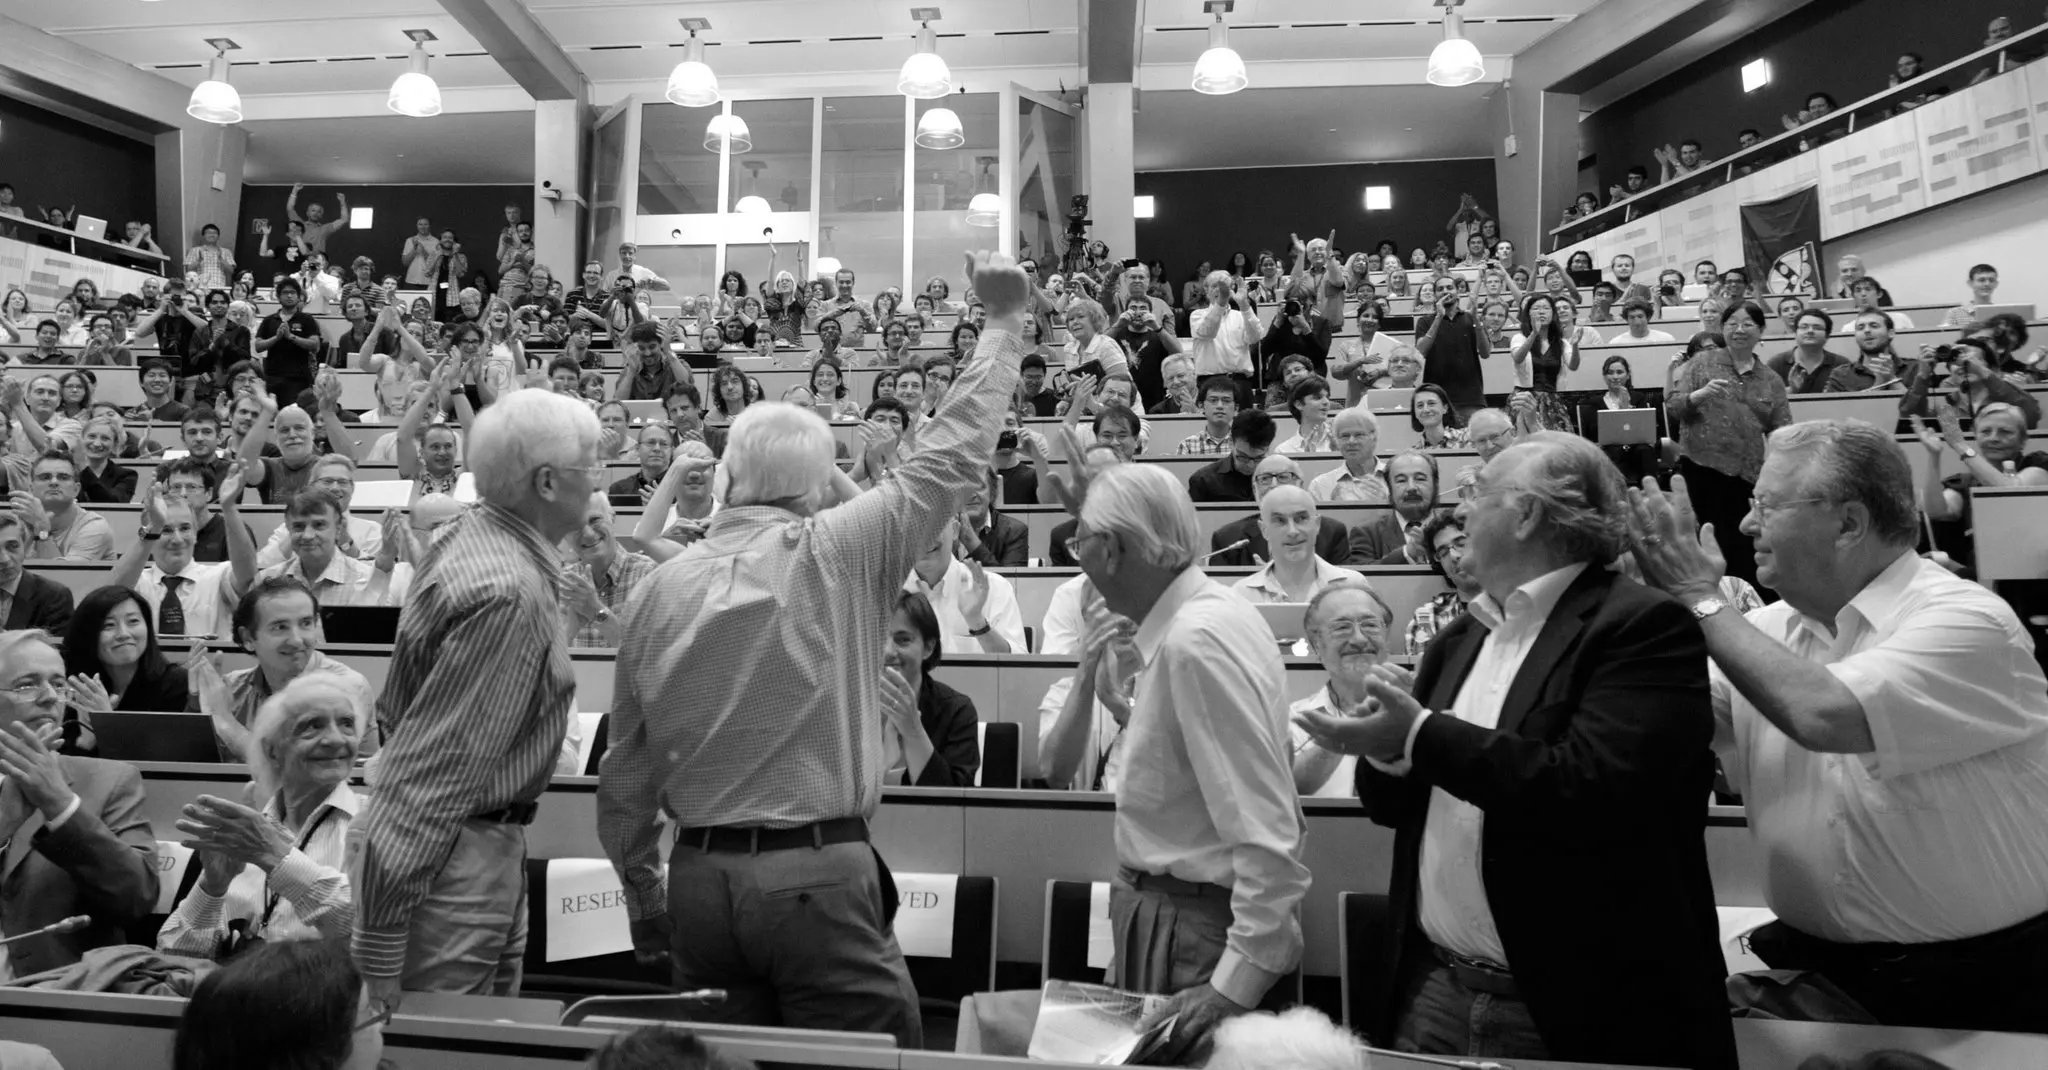
\includegraphics[width=0.5\textwidth]{./figures/HiggsBosonDiscoveryBW.png}
      \end{center}
    \end{figure}
    % ========================
  \end{multicols}
\end{MyArticle}
 \end{column}
    \end{columns}
\end{columns}

\begin{columns}[t]
  \begin{columns}[t,totalwidth=1.0\paperwidth] % split up that three-column-wide column
    \begin{column}{0.27\paperwidth} \begin{MyArticle}[enhanced, tikz={rotate=0}, boxrule=1pt,
  titlerule=0pt, width=0.33\textwidth]{CDF publishes multi-muons!}
  \begin{multicols}{2}
    We report a study of multi-muon events produced at the
    Fermilab Tevatron collider and recorded by the CDF~II detector. In a data 
    set acquired with a dedicated dimuon trigger and corresponding to an 
    integrated luminosity of 2100 pb$^{-1}$, we isolate a significant sample of 
    events in which at least one of the muon candidates is produced 
    outside of the beam pipe of radius 1.5 cm. The production cross section
    and kinematics of events in which both muon candidates are produced inside
    the beam pipe are successfully modeled by known QCD processes which
    include heavy flavor production. In contrast, we are presently unable to 
    fully account for the number and properties of the remaining events, in which
    at least one muon candidate is produced outside of the beam pipe, in terms
    of the same understanding of the CDF~II detector, trigger, and event 
    reconstruction. Several topological and kinematic properties of these 
    events are presented in this paper. These events offer a plausible 
    resolution to long-standing inconsistencies related to $b\bar{b}$
    production and decay.
    \begin{comment}
    % ========================
    \begin{figure}
      \begin{center}
        \vspace{-0.2in}
        \leavevmode
        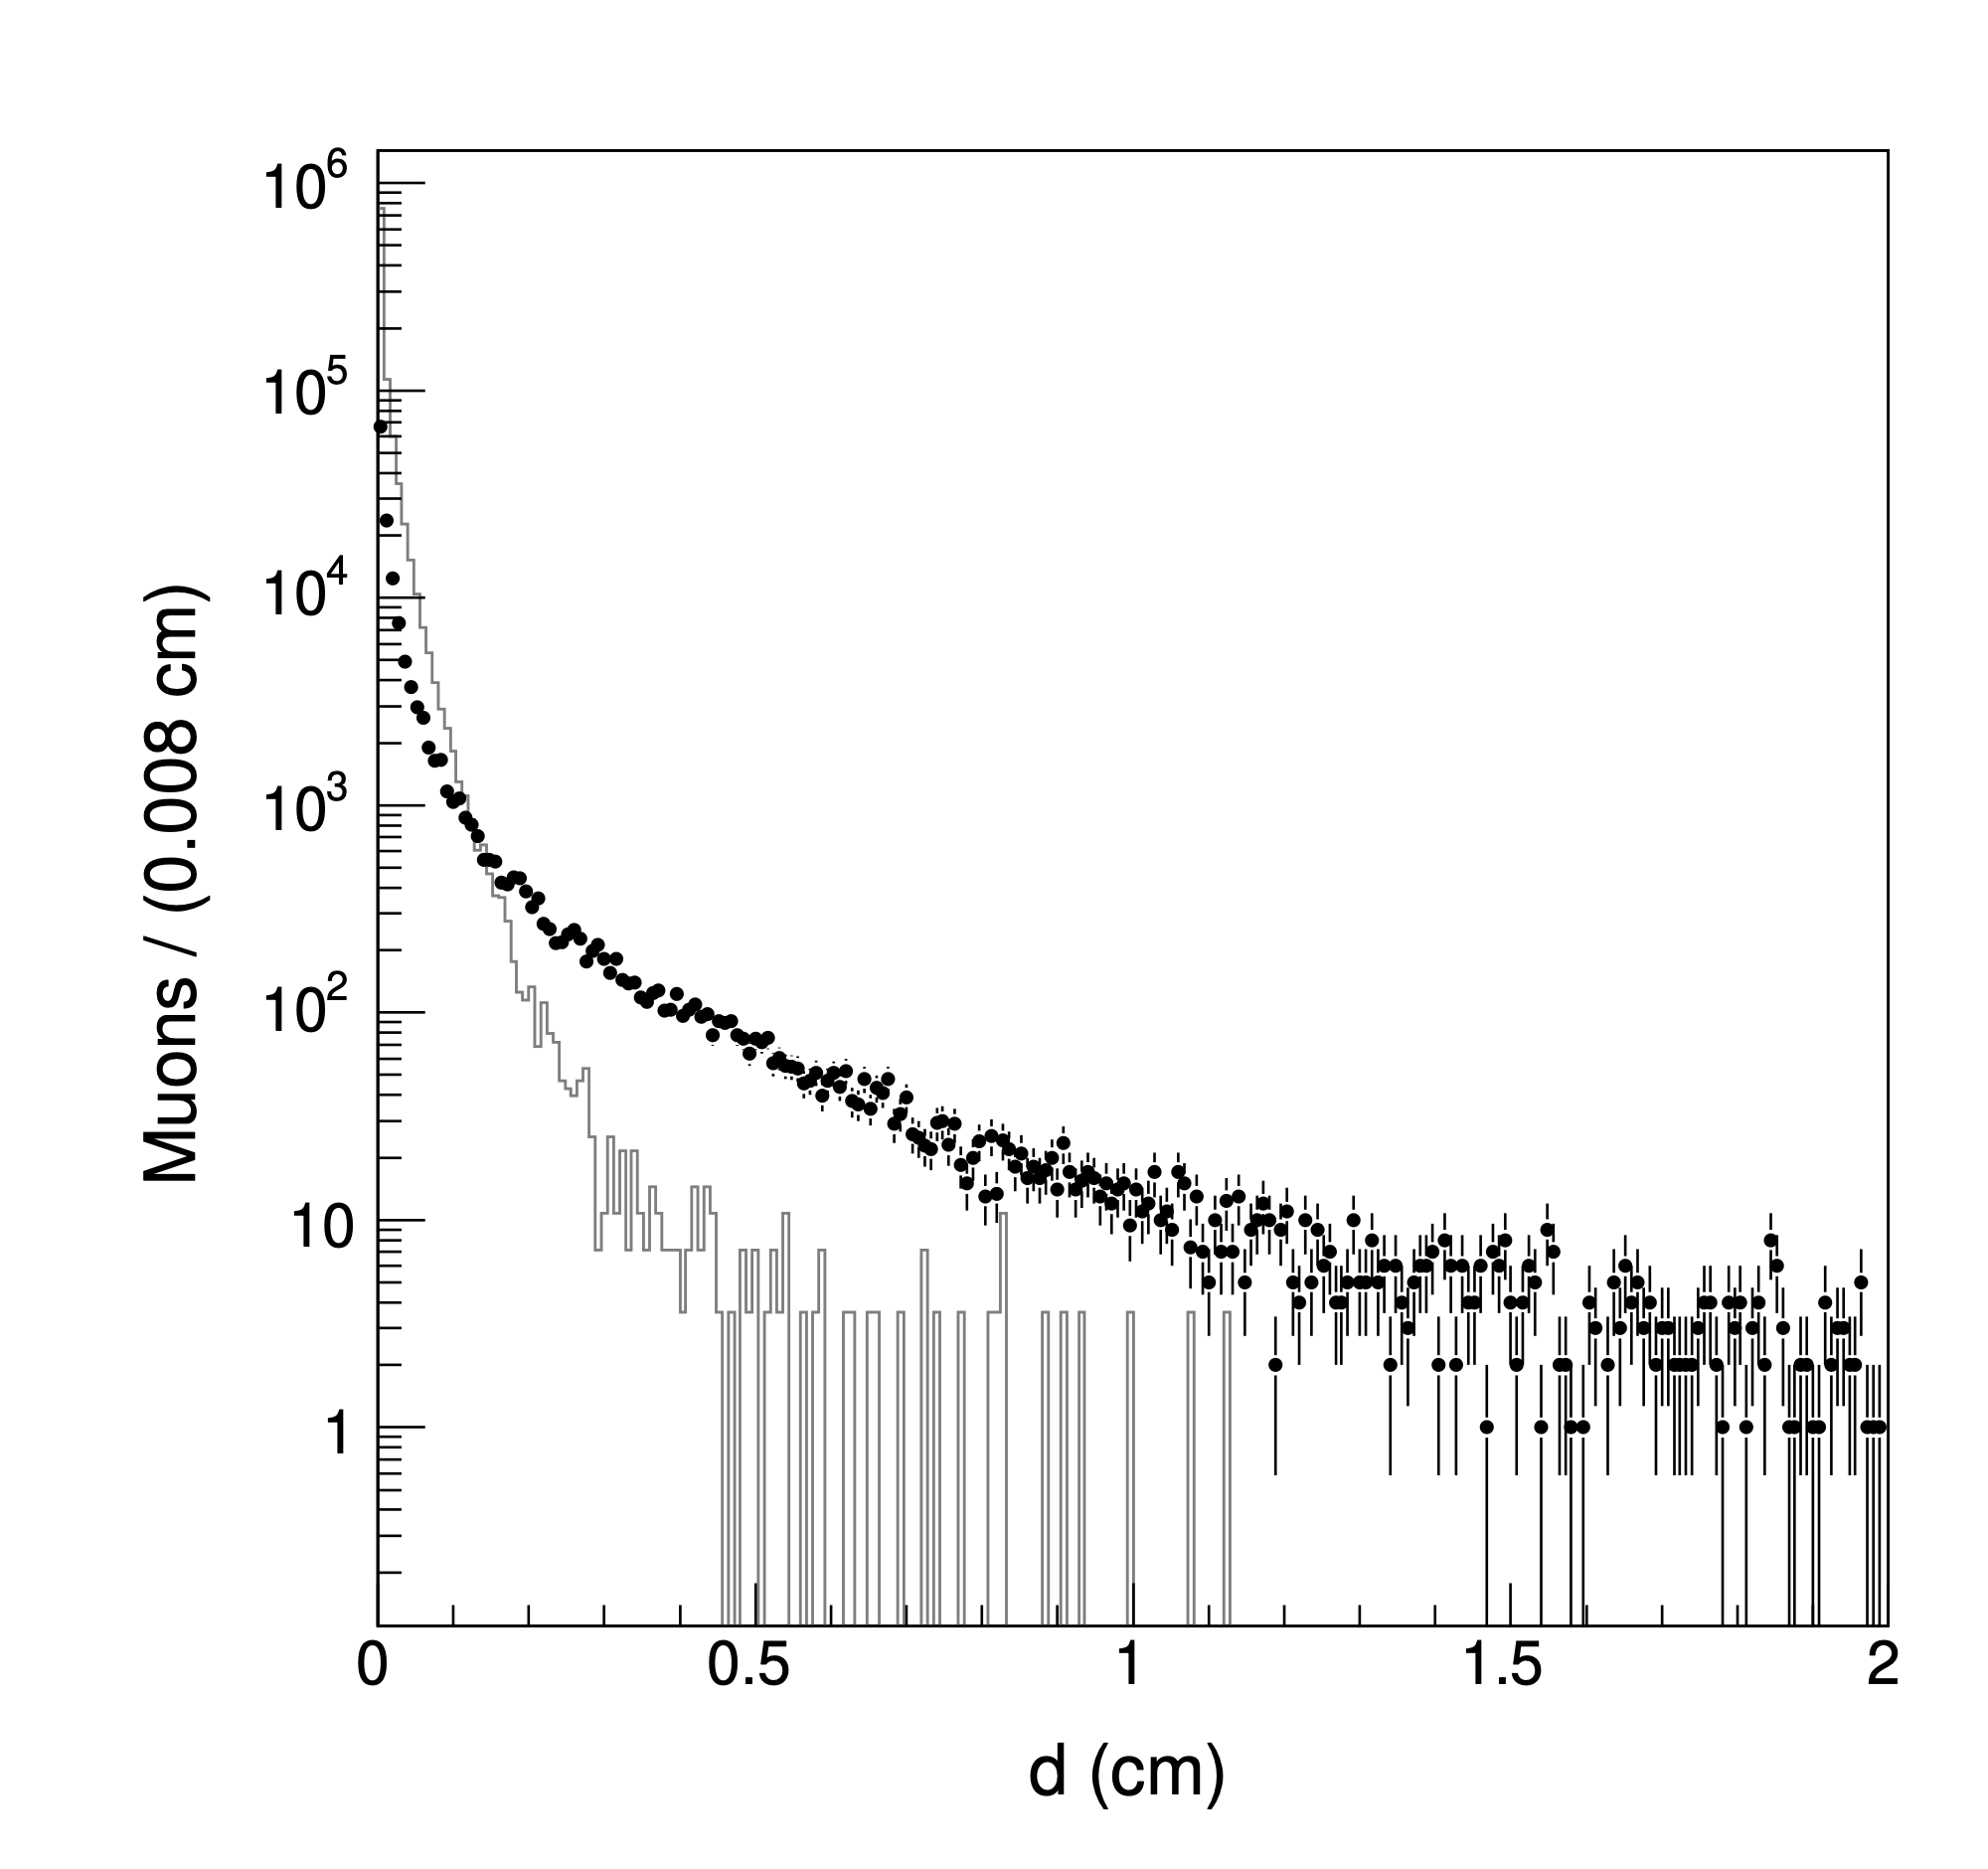
\includegraphics[width=\textwidth]{./figures/MultiMuons1BW_CDF.png}
        %\caption[] {Impact parameter distribution of muons contributed by ghost
        %  ($\bullet$) and QCD (histogram) events. Muon tracks are
        %  selected with loose SVX requirements. The detector resolution
        %  is $\simeq 30 \; \mu$m, whereas bins are 80 $\mu$m wide.} 
      \end{center}
    \end{figure}
    % ========================
    \end{comment}
  \end{multicols}
\end{MyArticle}
 \end{column}
    \begin{column}{0.27\paperwidth} % https://gitlab.cern.ch/tdr/papers/HIG-21-010/-/tree/master/
% new tcolorbox environment
\newtcolorbox{topQuark}[2][]{
  coltext      = black,
  colframe     = \MyBlockFrameColorLeft,
  colback      = \MyBlockFillColorLeft,
  colbacktitle = \MyBlockTitleBoxColor,
  coltitle     = black,
  title        = {\Large{\textbf{#2}}},
  fonttitle    = \bfseries,
  boxrule      = 0.2cm, %frame line width
  %tikz={rotate=#3}, % manipulate the tcolorbox as a whole (in degrees)
  top=+0.0cm, bottom=+0.0cm, left=+0.05cm, right=+0.05cm,
  %enlarge top by   = +1.0cm,  %  equivalent to mdframed 'skipabove'
  %enlarge bottom by= +0.0cm,  %  equivalent to mdframed 'skipbelow'
  %enlarge left by  = +1.5cm,  
  %enlarge right by = +0.0cm, 
  opacityback=1.0, % 1.0 means totally transparent, 0.0 means totally opaque
  arc=0.0cm,        % 0.0cm for non-rounded corners!
  #1,
}

% CMS
\begin{topQuark}[enhanced, tikz={rotate=0}]{Higgs boson: a tool to
    discover new physics: $H^{\pm}$}
  \begin{multicols}{2}
  A search for a charged Higgs boson $H^{\pm}$ decaying
  into a heavy neutral Higgs boson $H$ and a $W$ boson
  is presented. The analysis targets the $W$ decay into a pair
  of tau leptons with at least one of them decaying hadronically and
  with an additional electron or muon present in the event.
  The search is based on proton-proton collision data
  recorded by the CMS experiment during 2016--2018 at
  $\sqrt{s} = 13~TeV$, corresponding to an integrated
  luminosity of 138~$fb^{-1}$. The data are consistent with
  standard model background expectations. Upper limits at 95$\%$ confidence
  level are set on the product of the cross section and branching fraction
  for an $H^{\pm}$ in the mass range of 300--700 GeV, assuming an $H$ 
  with a mass of 200 GeV. The observed limits range from
  0.085 $pb$ for an $H^{\pm}$ mass of
  300 $GeV$ to 0.019~$pb$ for a mass of
  700 $GeV$. These are the first limits on $H^{\pm}$
  production in the $H^{\pm} \to H W^{\pm}$ decay channel at the LHC.
  \end{multicols}
\end{topQuark}
 \end{column}
    \begin{column}{0.4\paperwidth} \begin{MyArticle}[enhanced, tikz={rotate=0}]{Top Quark, Last Piece of Matter, Appears to Be in Place}
  \begin{multicols}{2}
    We establish the existence of the top quark using a 67 pb$^{-1}$ data
    sample of pp collisions at $\sqrt{s} = 1.8$ TeV collected with the Collider
    Detector at Fermilab (CDF). Employing techniques similar to those we
    previously published, we observe a signal consistent with $t\bar{t}$ decay to
    $WWbb$, but inconsistent with the background prediction by
    4.8$\sigma$. Additional evidence for the top quark is provided by a peak in
    the reconstructed mass distribution. We measure the top quark mass
    to be $176 \pm 8 (\text{stat.}) \pm 10 (\text{sys.})$ GeV/c$^{2}$,
    and the $t\bar{t}$ production cross section to be
    $6.8^{+3.6}_{-2.4}$ pb.
    % ========================
    \begin{figure}
      \begin{center}
        \vspace{-0.2in}
        \leavevmode
        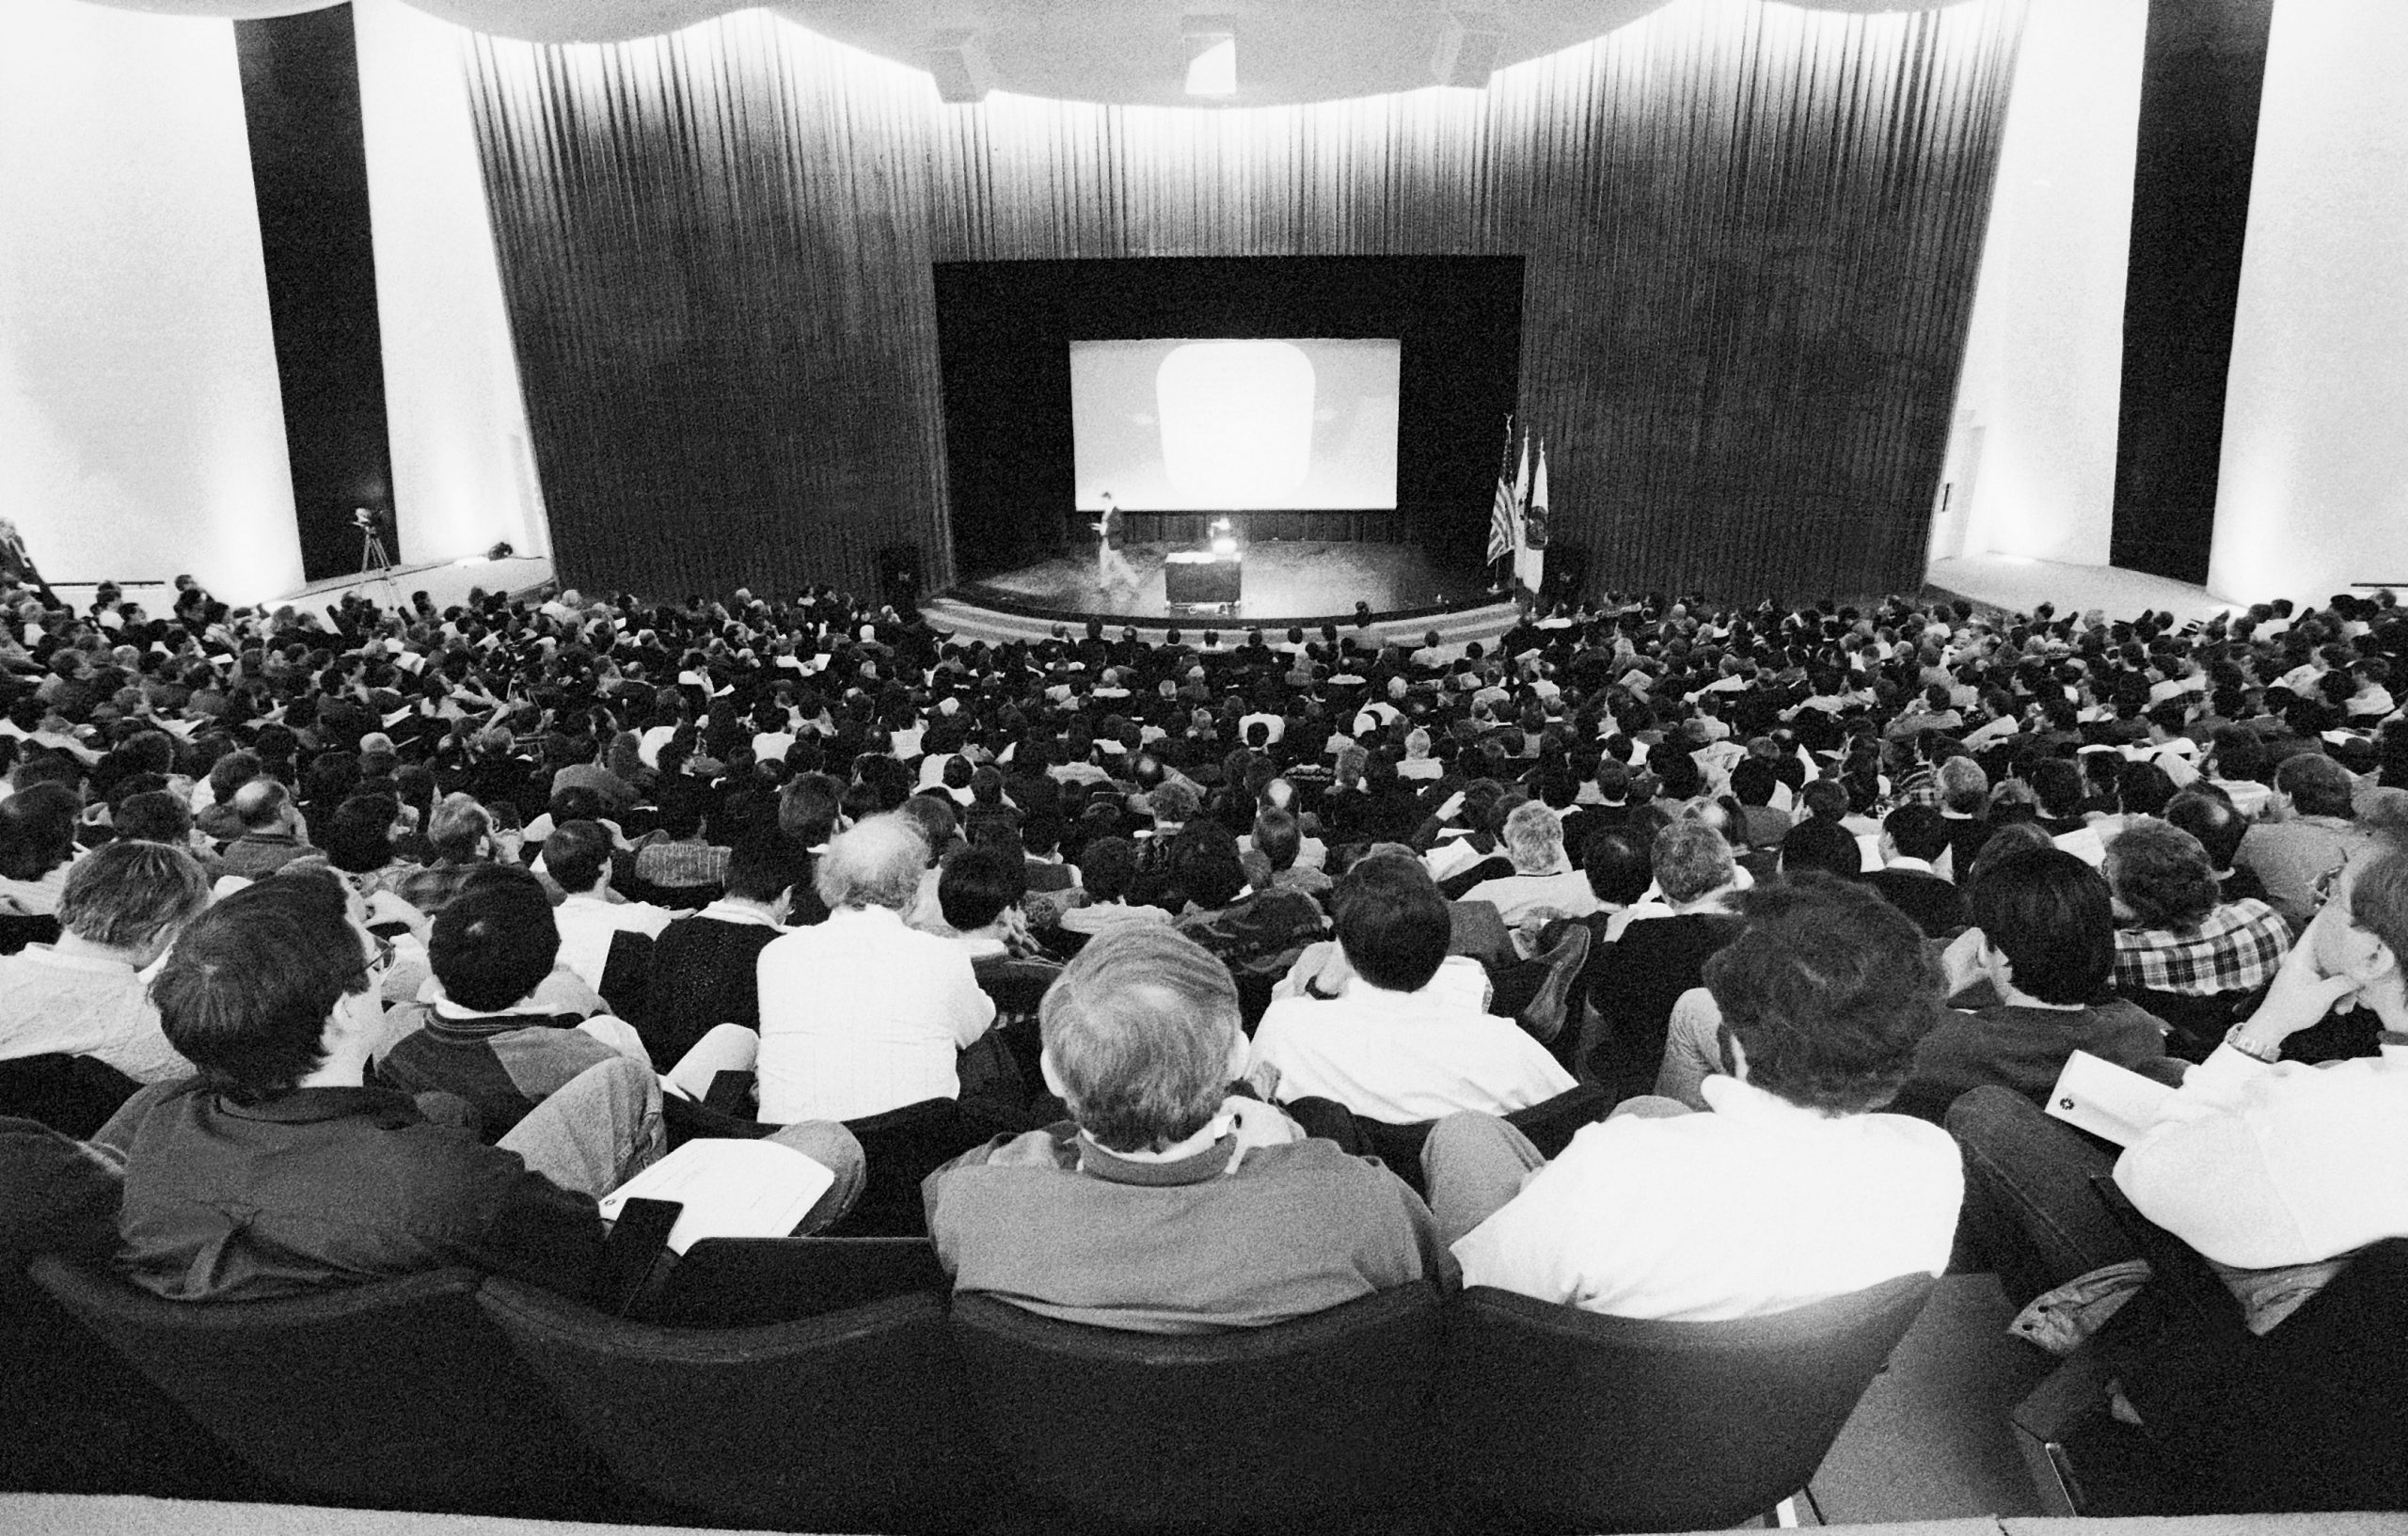
\includegraphics[width=0.5\textwidth]{./figures/TopQuarkAnnouncement.jpg}
      \end{center}
    \end{figure}
    % ========================
  \end{multicols}
\end{MyArticle}
 \begin{multimuons-2}[enhanced, tikz={rotate=0}]{Multi-Muons In CDF: The Mystery Continues}
  %\begin{multicols}{2}
    We present a phenomenological conjecture of new physics that is suggested
    by the topology and kinematic properties of the multi-muon events recently
    reported by the CDF collaboration. We show that the salient features of 
    the data can be accounted for by postulating the pair production of
    three new states $h_1$, $h_2$, and $h_3$ with masses in the range
    of 15, 7.3, and 3.6 GeV/c$^{2}$, respectively. The heavier states 
    cascade-decay into the lighter ones, whereas the lightest state 
    decays into a $\tau$ pair with a lifetime of the order of 20 ps.
    \begin{comment}
    % ========================
    \begin{figure}
      \begin{center}
        \vspace{-0.2in}
        \leavevmode
        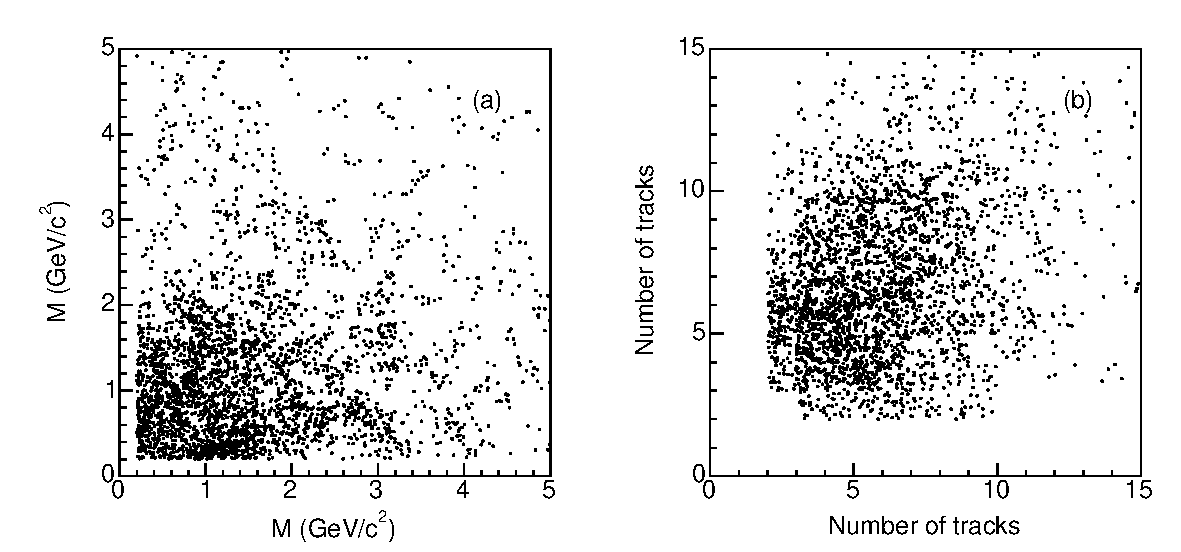
\includegraphics[width=\textwidth]{./figures/MultiMuons2_CDF.pdf}
        %\caption[]{Two-dimensional distributions, reproduced from Ref.~\cite{a0disc},
        %  of (a) the invariant mass, $M$, of all muons and (b) the total
        %  number of tracks contained in a $36.8^{\deg}$ cone when both
        %  cones contain at least two muons.}
      \end{center}
    \end{figure}
    % ========================
    \end{comment}
%  \end{multicols}
\end{multimuons-2}
\end{column}
  \end{columns}
\end{columns}
\end{comment}
%    \begin{columns}[t]
%    \begin{columns}[t,totalwidth=1.0\paperwidth] % split up that three-column-wide column
%      \begin{column}{0.25\paperwidth} \begin{MyArticle}[enhanced, tikz={rotate=0}, boxrule=1pt,
  titlerule=0pt, width=0.33\textwidth]{CDF publishes multi-muons!}
  \begin{multicols}{2}
    We report a study of multi-muon events produced at the
    Fermilab Tevatron collider and recorded by the CDF~II detector. In a data 
    set acquired with a dedicated dimuon trigger and corresponding to an 
    integrated luminosity of 2100 pb$^{-1}$, we isolate a significant sample of 
    events in which at least one of the muon candidates is produced 
    outside of the beam pipe of radius 1.5 cm. The production cross section
    and kinematics of events in which both muon candidates are produced inside
    the beam pipe are successfully modeled by known QCD processes which
    include heavy flavor production. In contrast, we are presently unable to 
    fully account for the number and properties of the remaining events, in which
    at least one muon candidate is produced outside of the beam pipe, in terms
    of the same understanding of the CDF~II detector, trigger, and event 
    reconstruction. Several topological and kinematic properties of these 
    events are presented in this paper. These events offer a plausible 
    resolution to long-standing inconsistencies related to $b\bar{b}$
    production and decay.
    \begin{comment}
    % ========================
    \begin{figure}
      \begin{center}
        \vspace{-0.2in}
        \leavevmode
        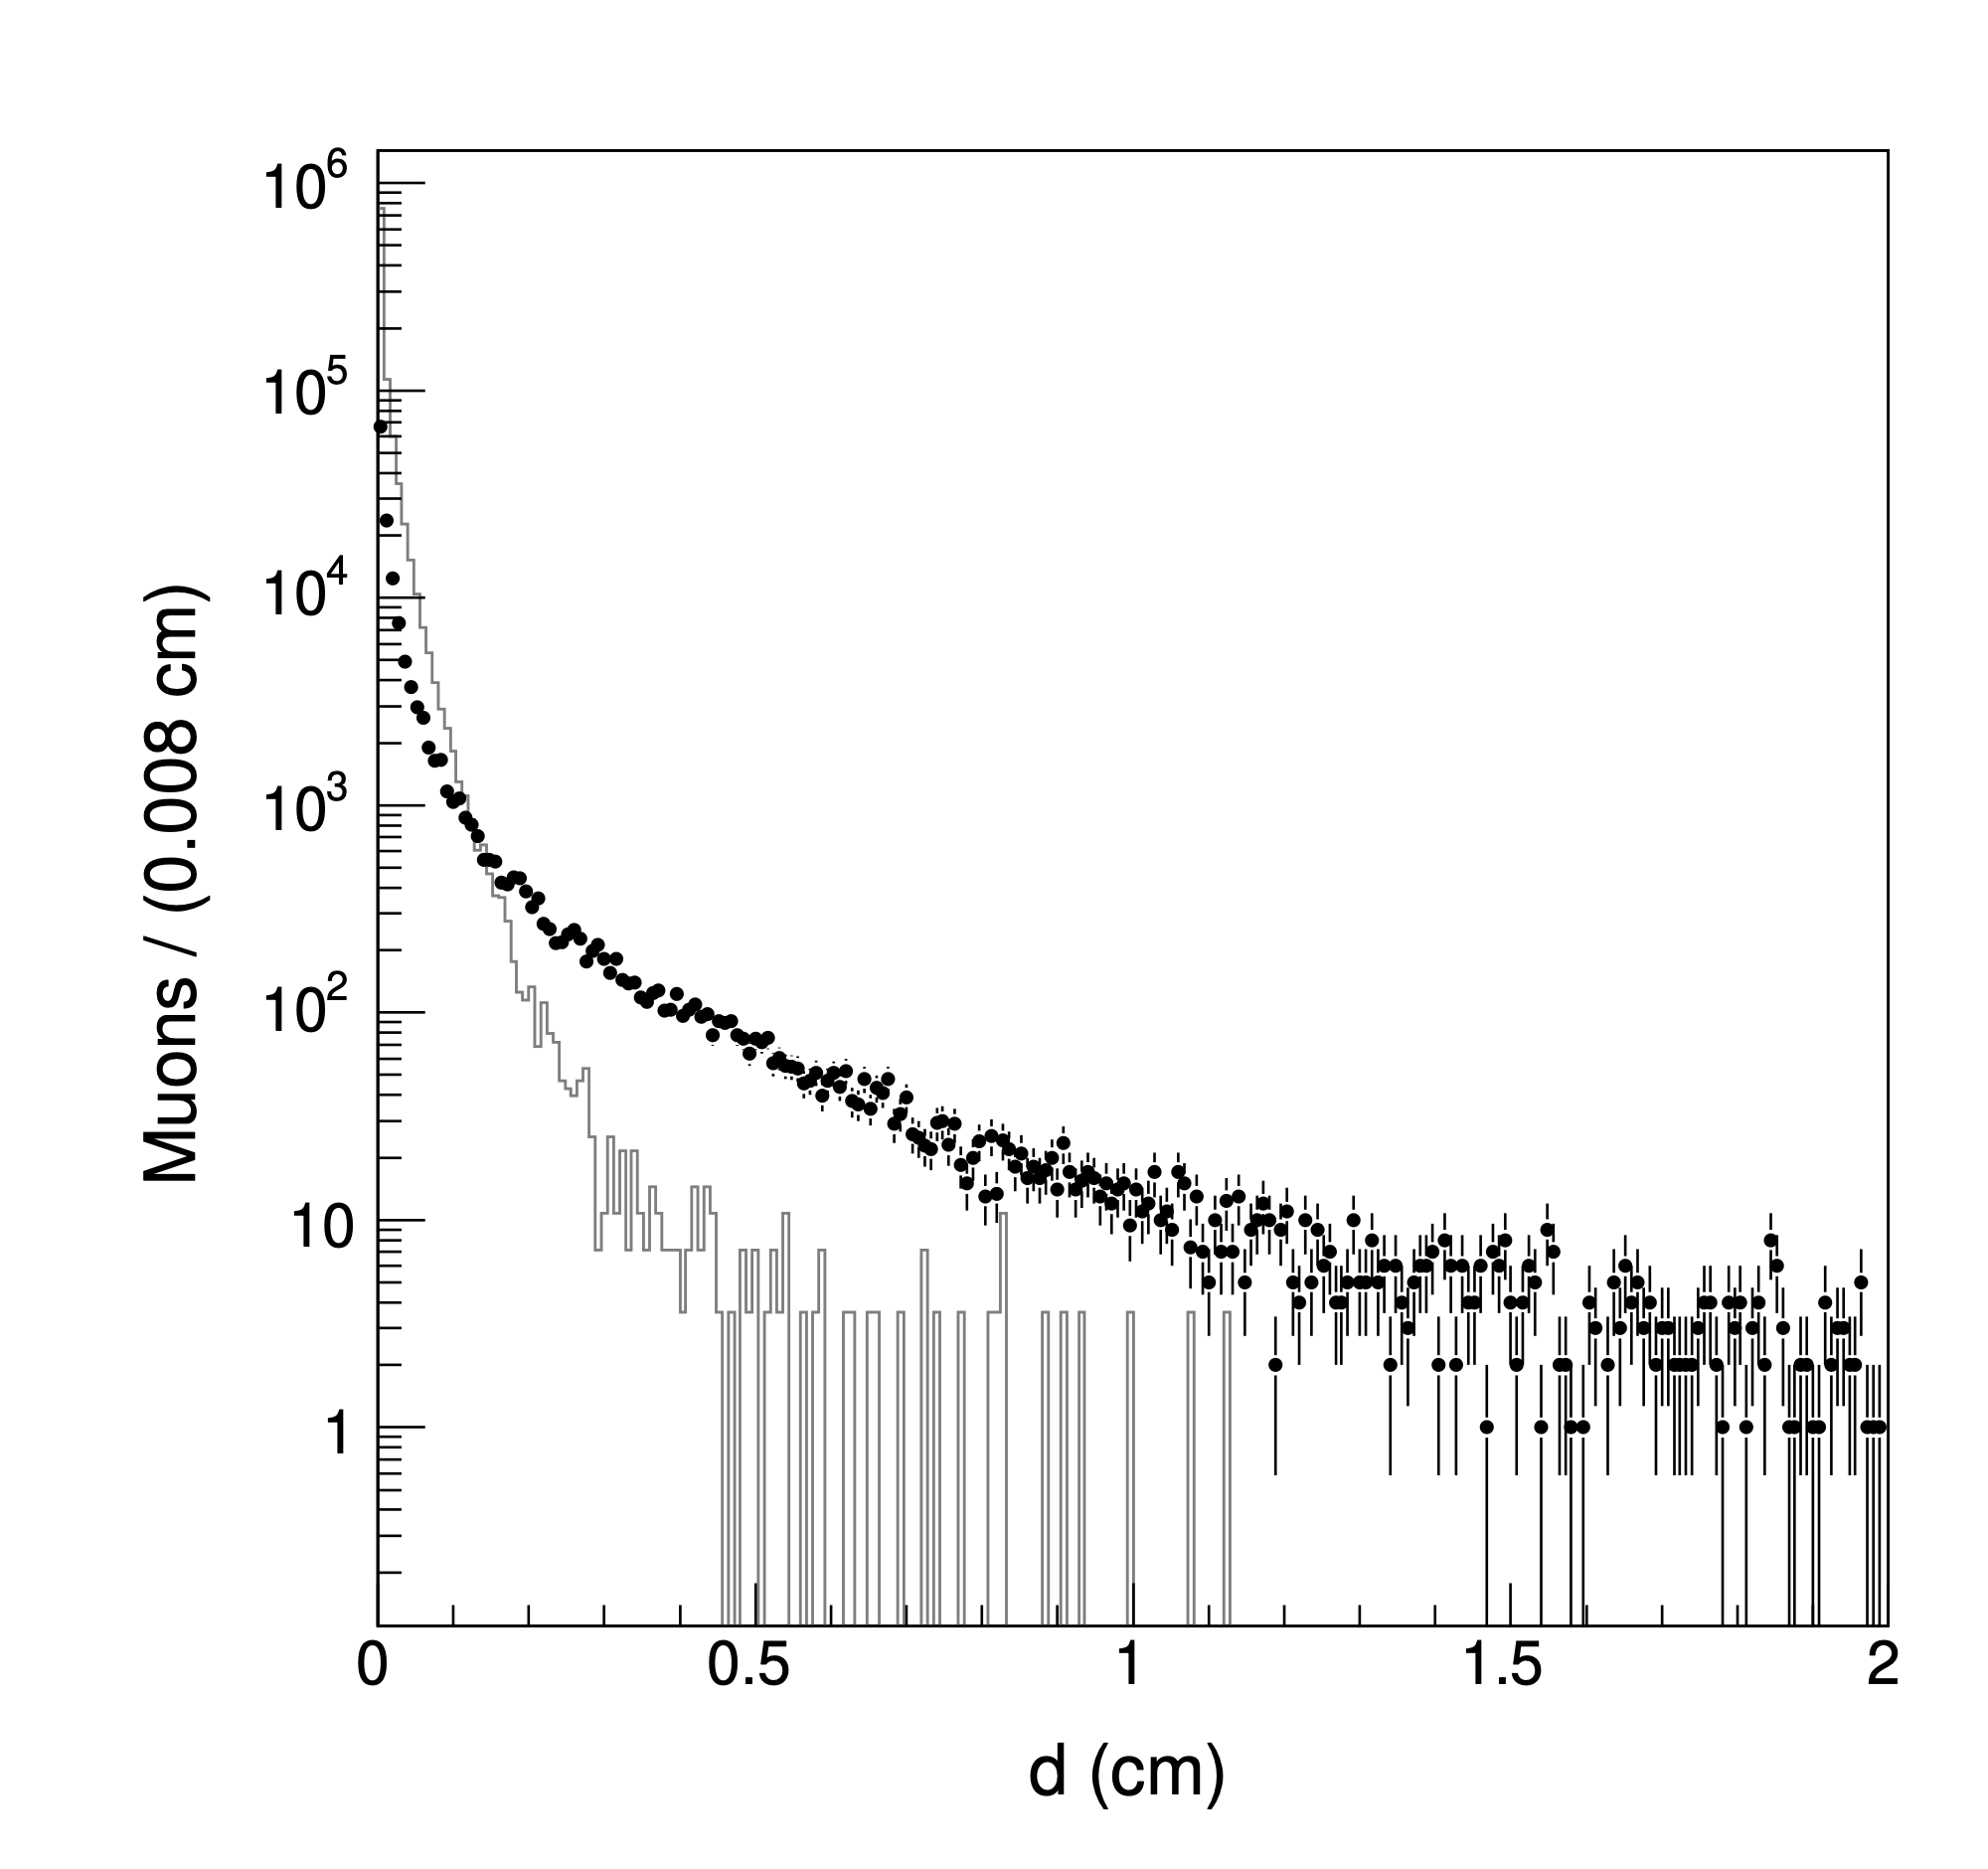
\includegraphics[width=\textwidth]{./figures/MultiMuons1BW_CDF.png}
        %\caption[] {Impact parameter distribution of muons contributed by ghost
        %  ($\bullet$) and QCD (histogram) events. Muon tracks are
        %  selected with loose SVX requirements. The detector resolution
        %  is $\simeq 30 \; \mu$m, whereas bins are 80 $\mu$m wide.} 
      \end{center}
    \end{figure}
    % ========================
    \end{comment}
  \end{multicols}
\end{MyArticle}
 \begin{MyArticle}[enhanced, tikz={rotate=0}, width=0.25\textwidth]{Charged Higgs boson
    Hunting}
  $t\rightarrow bH^{\pm}\rightarrow \tau^{\pm} \nu_{\tau}$............................\it{25 May 2012}\newline
  $H^{\pm}\rightarrow tb$ and $H^{\pm}\rightarrow \tau\nu$..............\it{31 August 2015}\newline
  $H^{\pm} \rightarrow \tau^{\pm} \nu_{\tau}$ ................................\it{11 March 2019}\newline
  $pp\rightarrow t(b)H^{\pm} \rightarrow tb$, all-jet.......\it{21 January 2020}\newline
  $pp\rightarrow t(b)H^{\pm} \rightarrow W^{\pm}H^{0}(\tau\tau)$...............\it{4 July 2022}
  %\begin{tabular}{l l}
%  \hline
%  \bf $H^{\pm} \rightarrow \tau^{\pm} \nu_{\tau}$  & \it{11 March 2019}\\
%  \bf $H^{\pm} \rightarrow tb$, all-jet            & \it{21 January 2020}\\
%  \bf $H^{\pm} \rightarrow W^{\pm}H^{0}(\tau\tau)$ & \it{4 July 2022}\\
%  \hline
%\end{tabular}
\end{MyArticle}
% https://cms-results.web.cern.ch/cms-results/public-results/publications/HIG-11-019/index.html
% https://cms-results.web.cern.ch/cms-results/public-results/publications/HIG-14-023/index.html
% https://cms-results.web.cern.ch/cms-results/public-results/publications/HIG-18-014/index.html
% https://cms-results.web.cern.ch/cms-results/public-results/publications/HIG-18-015/index.html
% https://cms-results.web.cern.ch/cms-results/public-results/publications/HIG-21-010/index.html


\begin{comment}
\begin{multimuons-1}[enhanced, tikz={rotate=0}, width=1.0\textwidth]{\huge Charged Higgs boson Hunting}

  \Large{$t\rightarrow bH^{\pm}\rightarrow \tau^{\pm} \nu_{\tau}$}............................\it{\Large 25 May 2012}\newline
  \Large{$H^{\pm}\rightarrow tb$ and $H^{\pm}\rightarrow \tau\nu$}..............\it{\Large 31 August 2015}\newline
  \Large{$H^{\pm} \rightarrow \tau^{\pm} \nu_{\tau}$}................................\it{\Large 11 March 2019}\newline
  \Large{$pp\rightarrow t(b)H^{\pm} \rightarrow tb$, all-jet}.......\it{\Large 21 January 2020}\newline
  \Large{$pp\rightarrow t(b)H^{\pm} \rightarrow W^{\pm}H^{0}(\tau\tau)$}...............\it{\Large 4 July 2022}
\end{multimuons-1}
\end{comment}
 \end{column}
%      \begin{column}{0.33\paperwidth} % new tcolorbox environment
\newtcolorbox{headline}[2][]{
  coltext      = black,
  colframe     = \MyBlockFrameColorLeft,
  colback      = \MyBlockFillColorLeft,
  colbacktitle = \MyBlockTitleBoxColor,
  coltitle     = black,
  title        = {\Huge{\textbf{#2}}},
  fonttitle    = \bfseries,
  boxrule      = 0.2cm, %frame line width
  %tikz={rotate=#3}, % manipulate the tcolorbox as a whole (in degrees)
  top=+0.0cm, bottom=+0.0cm, left=+0.05cm, right=+0.05cm,
  %enlarge top by   = +1.0cm,  %  equivalent to mdframed 'skipabove'
  %enlarge bottom by= +0.0cm,  %  equivalent to mdframed 'skipbelow'
  %enlarge left by  = +1.5cm,  
  %enlarge right by = +0.0cm, 
  opacityback=1.0, % 1.0 means totally transparent, 0.0 means totally opaque
  arc=0.0cm,        % 0.0cm for non-rounded corners!
  #1,
}

% CMS
\begin{headline}[enhanced, tikz={rotate=0}]{Fotios Ptochos Promoted to Professor!}
  \begin{multicols}{2}
    \lipsum[1]\\ 
    \lipsum[2]\\ 
    %\lipsum[3]\\ 
    % ========================
    \begin{figure}
      \begin{center}
        \vspace{-0.2in}
        \leavevmode
        \includegraphics[width=0.5\textwidth]{./figures/Fotis6.png}
      \end{center}
    \end{figure}
    % ========================
  \end{multicols}
\end{headline}
 \end{column}
%      \begin{column}{0.35\paperwidth} \begin{multimuons-2}[enhanced, tikz={rotate=0}]{Multi-Muons In CDF: The Mystery Continues}
  %\begin{multicols}{2}
    We present a phenomenological conjecture of new physics that is suggested
    by the topology and kinematic properties of the multi-muon events recently
    reported by the CDF collaboration. We show that the salient features of 
    the data can be accounted for by postulating the pair production of
    three new states $h_1$, $h_2$, and $h_3$ with masses in the range
    of 15, 7.3, and 3.6 GeV/c$^{2}$, respectively. The heavier states 
    cascade-decay into the lighter ones, whereas the lightest state 
    decays into a $\tau$ pair with a lifetime of the order of 20 ps.
    \begin{comment}
    % ========================
    \begin{figure}
      \begin{center}
        \vspace{-0.2in}
        \leavevmode
        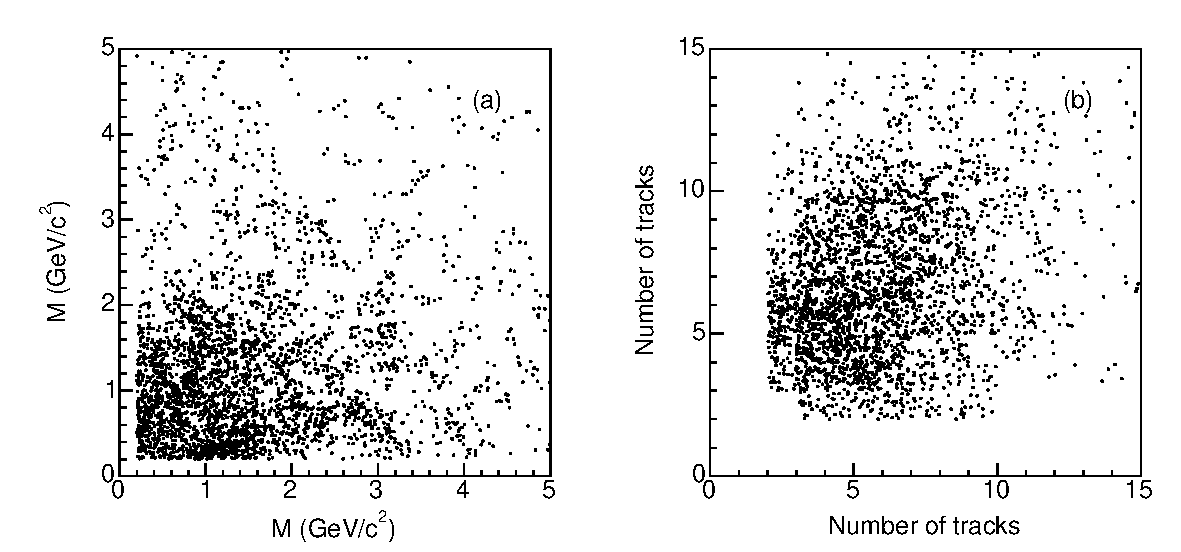
\includegraphics[width=\textwidth]{./figures/MultiMuons2_CDF.pdf}
        %\caption[]{Two-dimensional distributions, reproduced from Ref.~\cite{a0disc},
        %  of (a) the invariant mass, $M$, of all muons and (b) the total
        %  number of tracks contained in a $36.8^{\deg}$ cone when both
        %  cones contain at least two muons.}
      \end{center}
    \end{figure}
    % ========================
    \end{comment}
%  \end{multicols}
\end{multimuons-2}
 \end{column}
%    \end{columns}
%  \end{columns}


%\begin{columns}[t]
%    \begin{columns}[t,totalwidth=1.0\paperwidth] % split up that three-column-wide column
%      \begin{column}{0.35\paperwidth} \begin{MyArticle}[enhanced, tikz={rotate=0}]{Top Quark, Last Piece of Matter, Appears to Be in Place}
  \begin{multicols}{2}
    We establish the existence of the top quark using a 67 pb$^{-1}$ data
    sample of pp collisions at $\sqrt{s} = 1.8$ TeV collected with the Collider
    Detector at Fermilab (CDF). Employing techniques similar to those we
    previously published, we observe a signal consistent with $t\bar{t}$ decay to
    $WWbb$, but inconsistent with the background prediction by
    4.8$\sigma$. Additional evidence for the top quark is provided by a peak in
    the reconstructed mass distribution. We measure the top quark mass
    to be $176 \pm 8 (\text{stat.}) \pm 10 (\text{sys.})$ GeV/c$^{2}$,
    and the $t\bar{t}$ production cross section to be
    $6.8^{+3.6}_{-2.4}$ pb.
    % ========================
    \begin{figure}
      \begin{center}
        \vspace{-0.2in}
        \leavevmode
        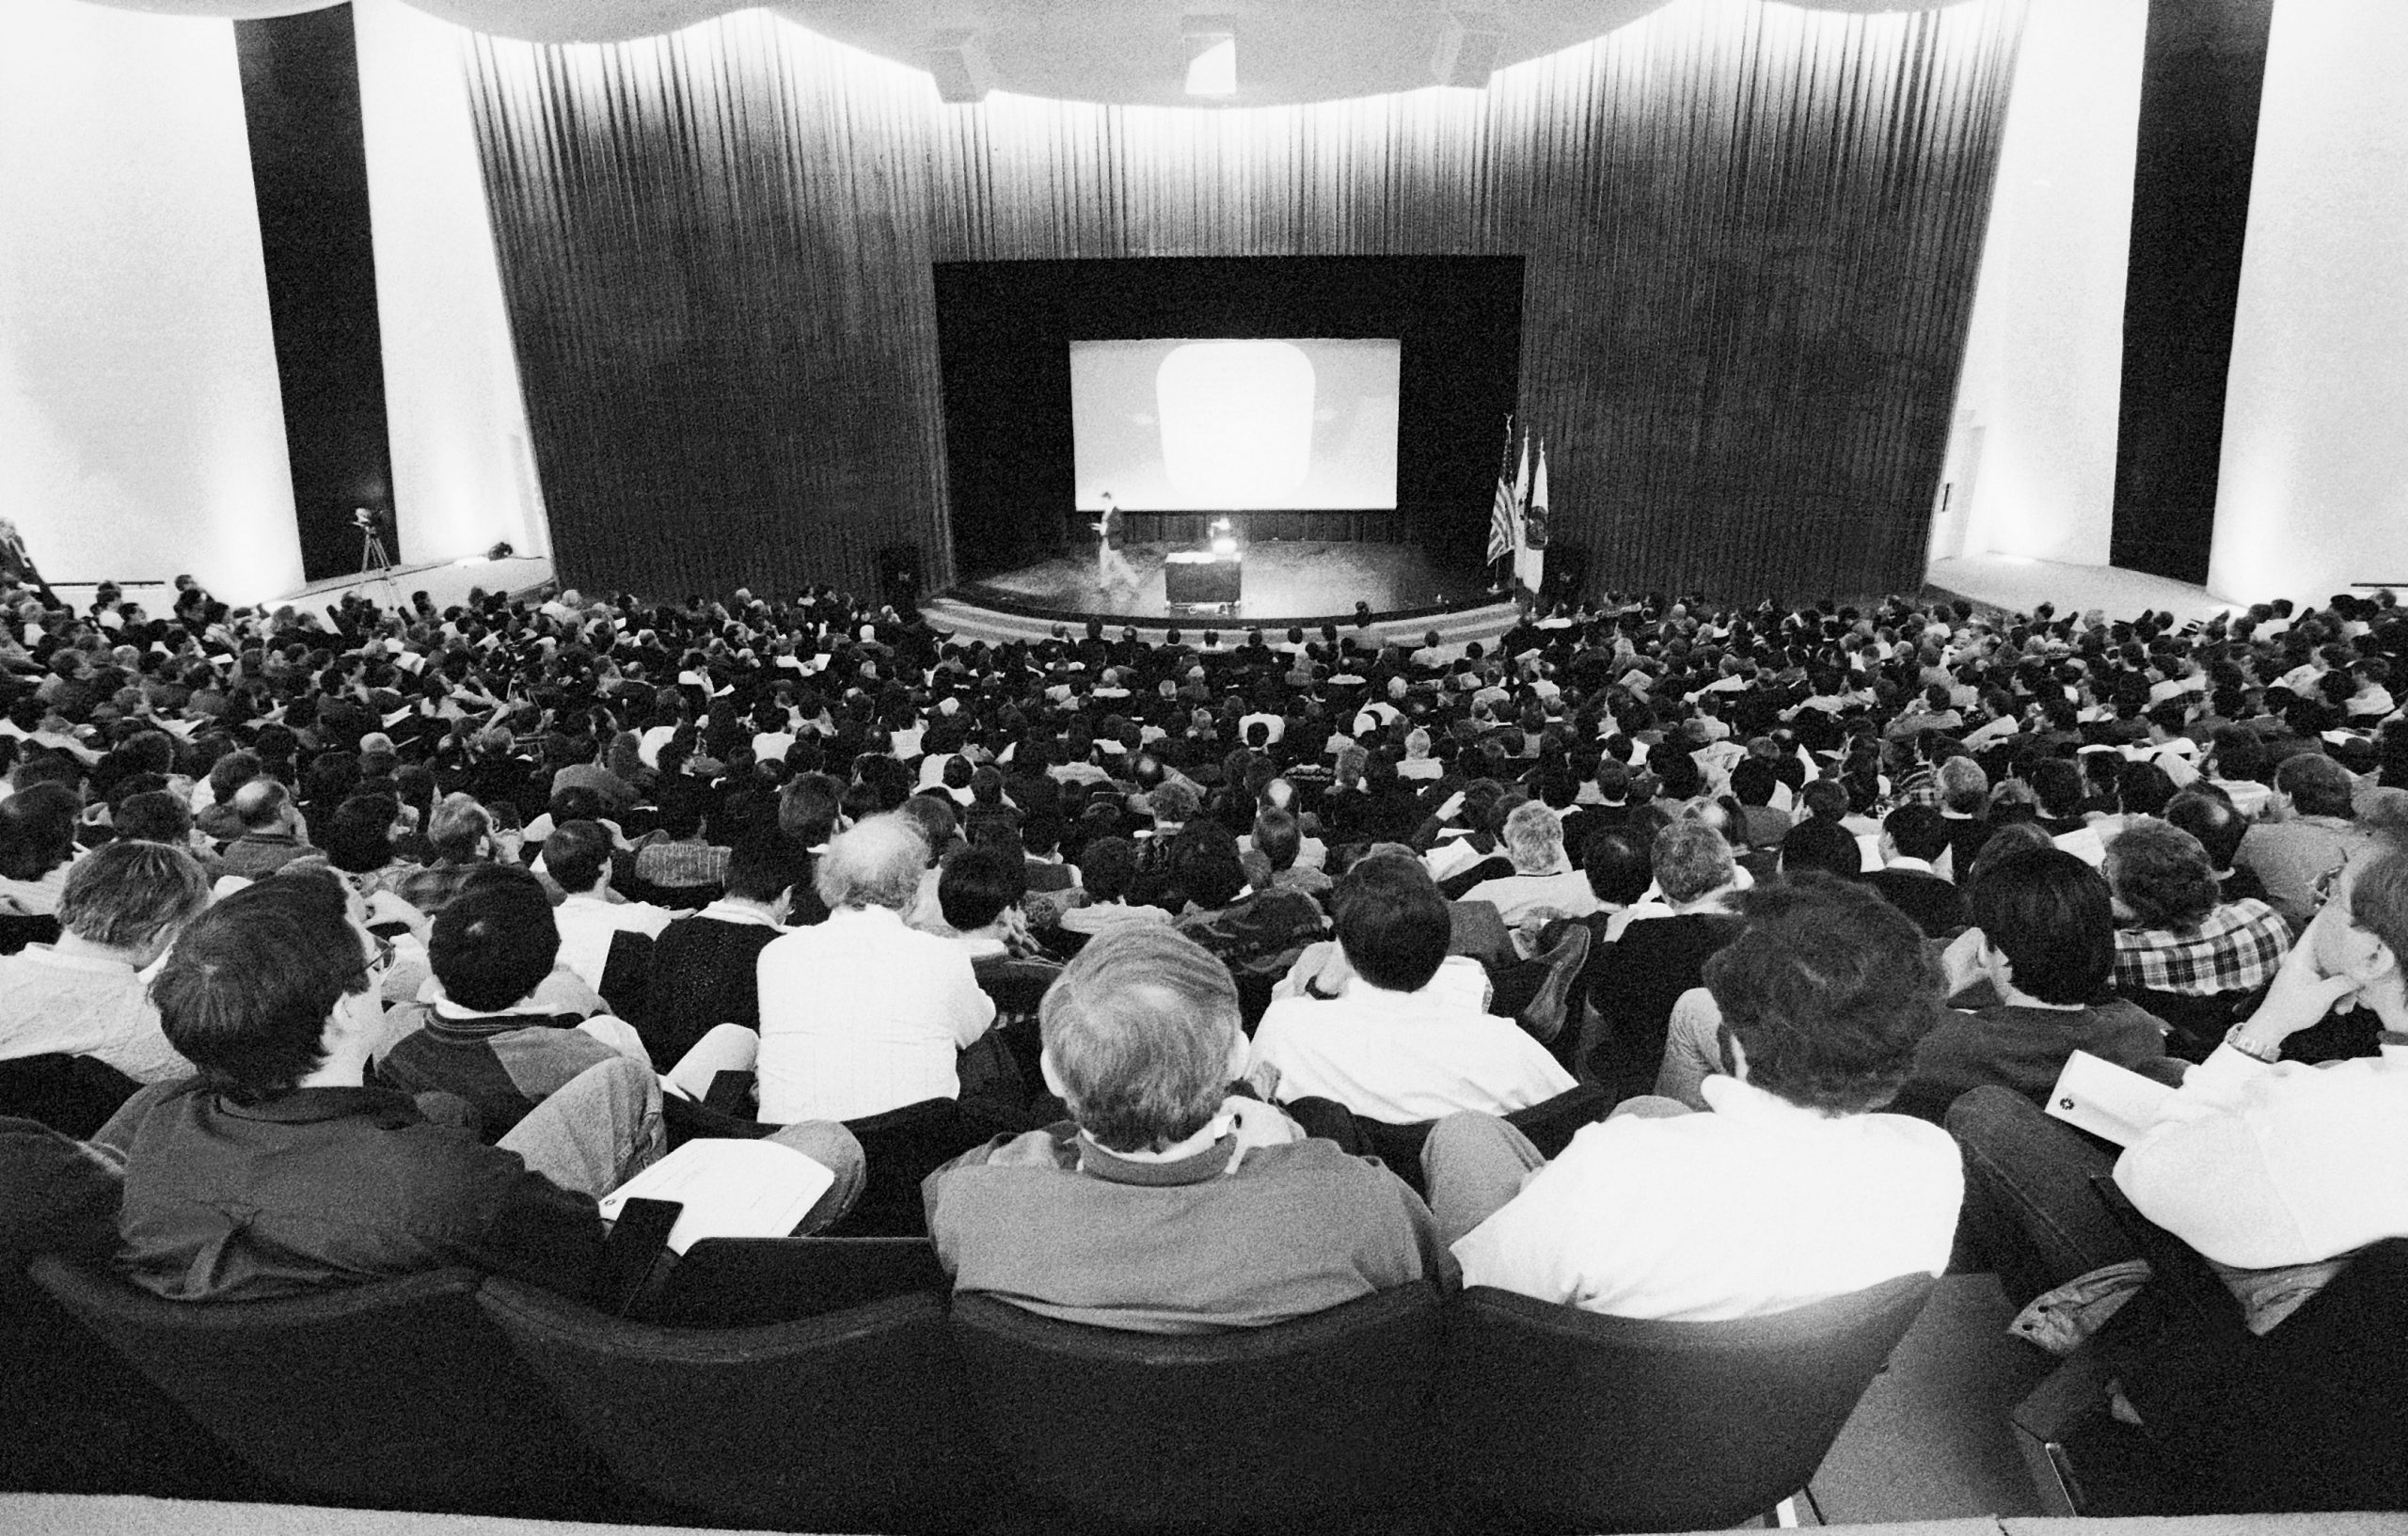
\includegraphics[width=0.5\textwidth]{./figures/TopQuarkAnnouncement.jpg}
      \end{center}
    \end{figure}
    % ========================
  \end{multicols}
\end{MyArticle}
 \end{column}
%      \begin{column}{0.35\paperwidth}  %\begin{MyArticle}[enhanced, height=0.2\textheight,
%tikz={rotate=0}]{Physicists Find Elusive Particle Seen as Key to
%Universe}
\begin{MyArticle}[enhanced, tikz={rotate=0}, width=0.35\textwidth]{Physicists Find Elusive Particle Seen as Key to Universe}
  \begin{multicols}{2}
    Results are presented from searches for the standard model Higgs
    boson in proton–proton collisions at and 8 TeV in the Compact Muon
    Solenoid experiment at the LHC, using data samples corresponding
    to integrated luminosities of up to 5.1 fb$^{−1}$ at 7 TeV and 5.3 fb$^{−1}$
    at 8 TeV. The search is performed in five decay modes:
    $\gamma\gamma$, $ZZ$,  $\tau^{+}\tau^{-}$, and $b\bar{b}$.
    An excess of events is observed above the expected background,
    with a local significance of 5.0 standard deviations, at a mass
    near 125 GeV, signalling the production of a new particle. The
    expected significance for a standard model Higgs boson of that
    mass is 5.8 standard deviations. The excess is most significant in
    the two decay modes with the best mass resolution, $\gamma\gamma$ and $ZZ$; a
    fit to these signals gives a mass of 
    $125.3\pm0.4(\text{stat.})\pm0.5(\text{syst.}$ GeV. The decay to
    two photons indicates that the new particle is a boson with spin 
    different from one. 
    % ========================
    \begin{figure}
      \begin{center}
        \vspace{-0.2in}
        \leavevmode
        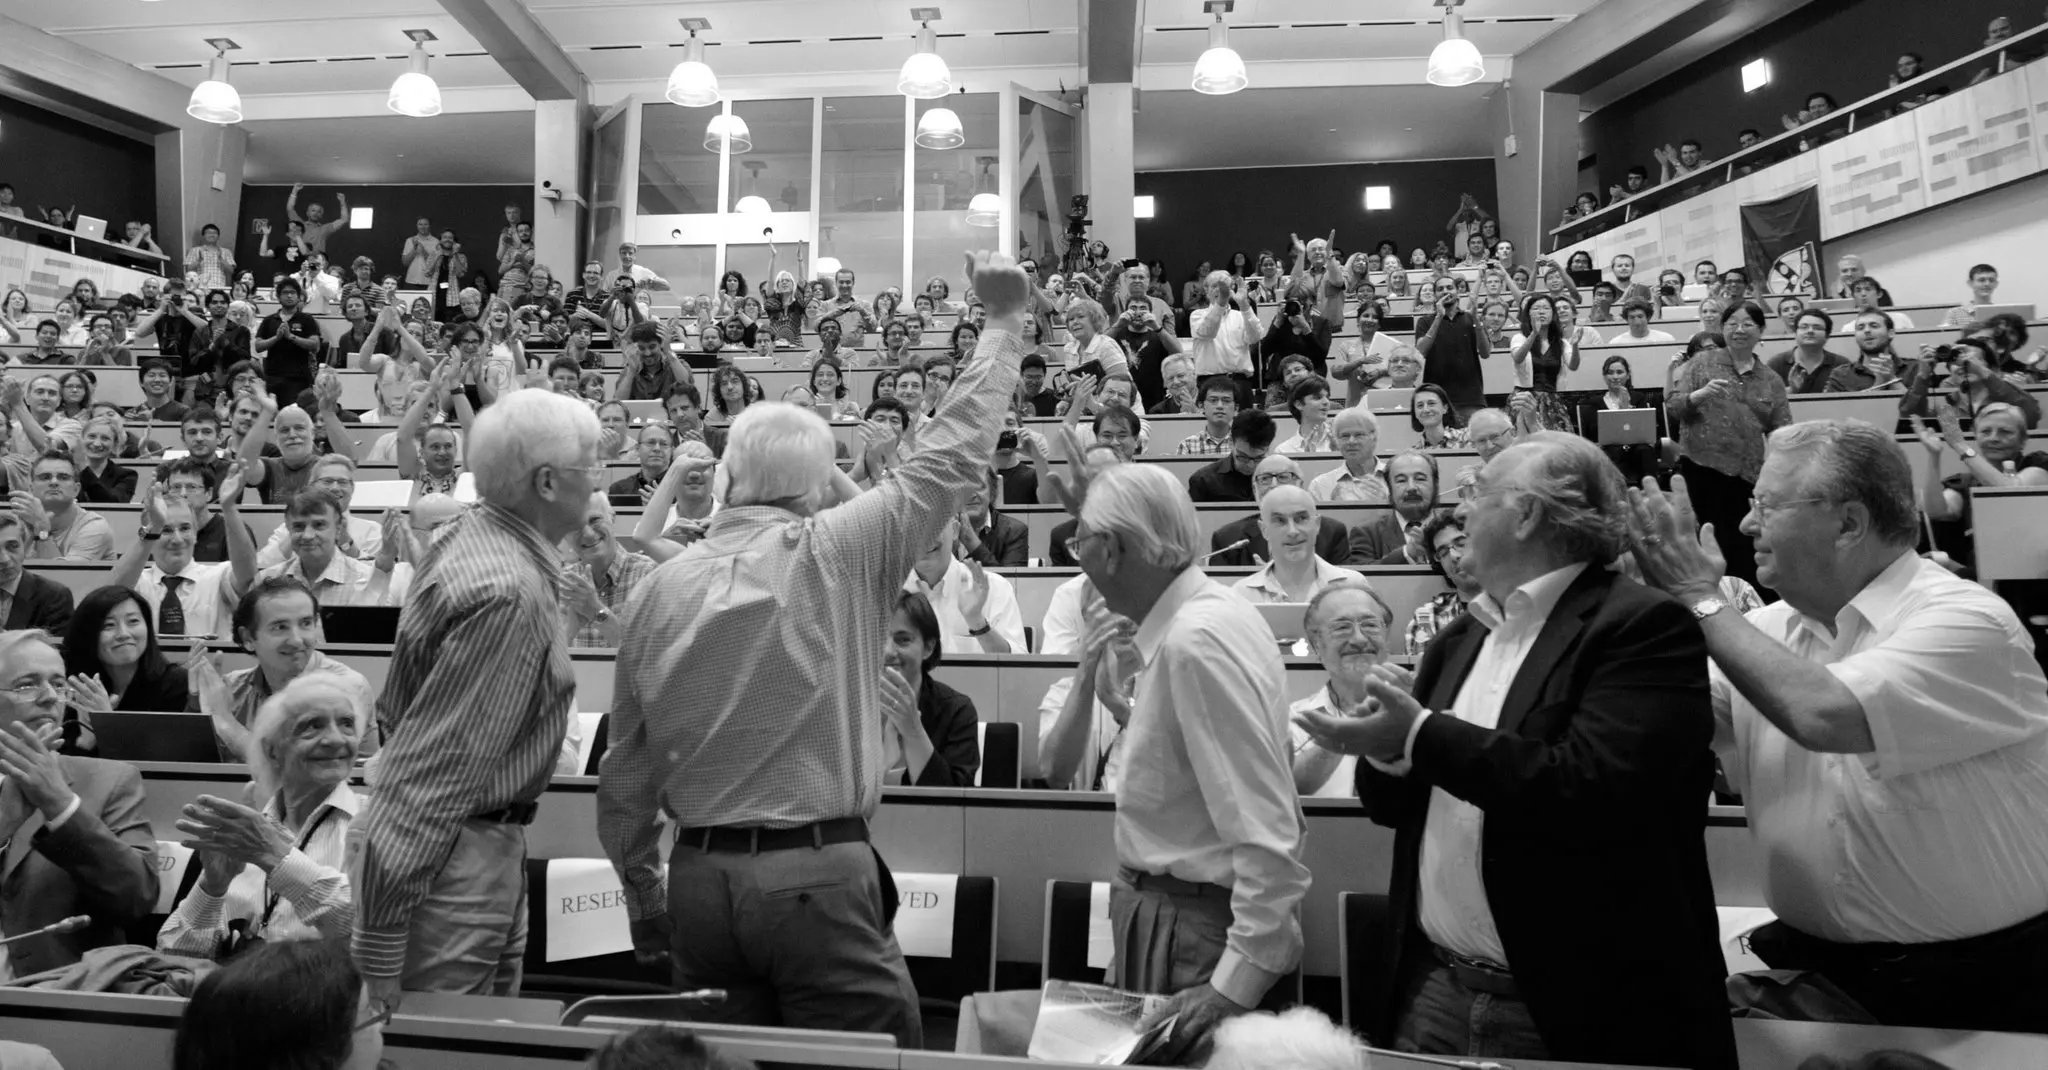
\includegraphics[width=0.5\textwidth]{./figures/HiggsBosonDiscoveryBW.png}
      \end{center}
    \end{figure}
    % ========================
  \end{multicols}
\end{MyArticle}
 \end{column}
%      \begin{column}{0.25\paperwidth} % https://gitlab.cern.ch/tdr/papers/HIG-21-010/-/tree/master/
% new tcolorbox environment
\newtcolorbox{topQuark}[2][]{
  coltext      = black,
  colframe     = \MyBlockFrameColorLeft,
  colback      = \MyBlockFillColorLeft,
  colbacktitle = \MyBlockTitleBoxColor,
  coltitle     = black,
  title        = {\Large{\textbf{#2}}},
  fonttitle    = \bfseries,
  boxrule      = 0.2cm, %frame line width
  %tikz={rotate=#3}, % manipulate the tcolorbox as a whole (in degrees)
  top=+0.0cm, bottom=+0.0cm, left=+0.05cm, right=+0.05cm,
  %enlarge top by   = +1.0cm,  %  equivalent to mdframed 'skipabove'
  %enlarge bottom by= +0.0cm,  %  equivalent to mdframed 'skipbelow'
  %enlarge left by  = +1.5cm,  
  %enlarge right by = +0.0cm, 
  opacityback=1.0, % 1.0 means totally transparent, 0.0 means totally opaque
  arc=0.0cm,        % 0.0cm for non-rounded corners!
  #1,
}

% CMS
\begin{topQuark}[enhanced, tikz={rotate=0}]{Higgs boson: a tool to
    discover new physics: $H^{\pm}$}
  \begin{multicols}{2}
  A search for a charged Higgs boson $H^{\pm}$ decaying
  into a heavy neutral Higgs boson $H$ and a $W$ boson
  is presented. The analysis targets the $W$ decay into a pair
  of tau leptons with at least one of them decaying hadronically and
  with an additional electron or muon present in the event.
  The search is based on proton-proton collision data
  recorded by the CMS experiment during 2016--2018 at
  $\sqrt{s} = 13~TeV$, corresponding to an integrated
  luminosity of 138~$fb^{-1}$. The data are consistent with
  standard model background expectations. Upper limits at 95$\%$ confidence
  level are set on the product of the cross section and branching fraction
  for an $H^{\pm}$ in the mass range of 300--700 GeV, assuming an $H$ 
  with a mass of 200 GeV. The observed limits range from
  0.085 $pb$ for an $H^{\pm}$ mass of
  300 $GeV$ to 0.019~$pb$ for a mass of
  700 $GeV$. These are the first limits on $H^{\pm}$
  production in the $H^{\pm} \to H W^{\pm}$ decay channel at the LHC.
  \end{multicols}
\end{topQuark}
 \end{column}
%    \end{columns}
%  \end{columns}

